% \documentclass[openany]{book}
\documentclass[10pt,a4paper]{report} 
\usepackage[utf8]{inputenc}
\usepackage{polski}
\usepackage{babel}
\usepackage{enumerate}
\usepackage{graphicx, caption}
\usepackage{listings,mdframed}
\usepackage{fontawesome}
\usepackage{mdframed}
\usepackage{multicol}
\usepackage[left=0.5in,right=0.5in,top=2cm, bottom=4cm]{geometry}
\usepackage{changepage}
\usepackage{sidecap}
\usepackage{pifont}

\usepackage{hyperref}

\renewcommand{\lstlistlistingname}{Spis listingów}

\begin{document}
\begin{flushleft}

\includegraphics[width=200px]{img/UMCS_skrocone_12G_PL_gray}

\vspace{1cm}
\begin{adjustwidth}{1.5in}{0cm}
\Large 
UNIWERSYTET MARII CURIE-SKŁODOWSKIEJ \\ W LUBLINIE \\
Wydział Matematyki, Fizyki i Informatyki
\end{adjustwidth}

\vspace{1cm}
\begin{adjustwidth}{1.2in}{0cm}

\begin{mdframed}[linewidth=0.5, topline=false,rightline=false,bottomline=false]
\normalsize 
\vspace{0.5cm}
 Kierunek: Informatyka 
 
 \vspace{1cm}
 
 \textbf{Mariia Sydor} \\ 
 nr albumu:296592 
 
 \vspace{2cm}
 \Large
 \textbf{Projekt i implementacja aplikacji dydaktycznej wspierającej naukę obsługi konsoli Linux.} \\

\vspace{0.5cm}

\normalsize 
\textbf{Design and implementation of a didactic application supporting the \\ learning of the linux console.} 
\vspace{2cm}
 
 Praca licencjacka \\
 napisana w Katedrze Cyberbezpieczeństwa \\
 pod kierunkiem dr Anety Wróblewskiej
 \vspace{0.5cm}
 
\end{mdframed}

\vspace{1cm}
\begin{adjustwidth}{0.5cm}{0cm}
\textbf{Lublin  rok 2022}
\end{adjustwidth}
\thispagestyle{empty}
\end{adjustwidth}
\end{flushleft}

\normalsize 

\begin{adjustwidth}{2cm}{2cm}
\tableofcontents
\chapter*{Wstęp}
\addcontentsline{toc}{chapter}{Wstęp}
\begin{minipage}{1\linewidth}
Konsola jest narzędzie o olbrzymich możliwościach. Wie o tym tylko ten, kto korzystał z niej przez dłuższą chwilę. Wiersz poleceń systemu Linux to interfejs tekstowy. Znany również jako powłoka, terminal, konsola i wiele innych, to program komputerowy przeznaczony do interpretowania poleceń. \\ \\
Linux to jeden z najczęściej używanych systemów operacyjnych, stanowiący podstawę wszystkiego, od komputerów PC po serwery i telefony komórkowe. Istnieje on od lat 90 i jest używany na całym świecie, w każdej możliwej do wyobrażenia aplikacji i dziedzinie. Niestety opinia publiczna nie jest zbyt zaznajomiona ze słowem Linux, mimo że Linux od dziesięcioleci zapewnia on niezawodność i bezpieczeństwo związane z systemem operacyjnym. \\ \\
Celem niniejszej pracy jest stworzenie dydaktycznej aplikacji wspierającej naukę obsługi konsoli Linux, która uprościłaby zwykłym użytkownikom naukę podstaw terminala Linux, bez konieczności instalowania systemu Linux lub uruchamiania go na wirtualnej maszynie, aby korzystać z aplikacji wystarczy że użytkownik uruchomi ją u siebie w przeglądarce. \\ \\
W pierwszym rozdziale wprowadzono czytelnika do ogólnych informacji na temat Linuksa oraz terminala. W kolejnym przedstawione zostały wykorzystane do napisania aplikacji narzędzia.
Ostatni rozdział poświęcono na opisanie powstałej aplikacji. Przedstawione zostały założenia aplikacji, omówienie poszczególnych przypadków użycia oraz tabel bazy danych. Następnie zostały omówione wybrane fragmenty kody, części frontendowej aplikacji. Na końcu zaprezentowano wygląd aplikacji.
\end{minipage}
\chapter{Wprowadzenie}
\section{Linux}
\begin{minipage}{1\linewidth}
Linux stanowi jedną z wersji systemu operacyjnego należącego do rodziny systemów uniksowych.
Podobnie jak inne systemy, takie jak Windows, macOS, Linux posiada interfejs graficzny i te same typy oprogramowania, takie jak edytory tekstu, zdjęć, video itp. \\ \\
Różni się również pod wieloma względami od innych systemów. Po pierwsze Linux jest oprogramowaniem open source. Jego kod jest darmowy i publicznie dostępny do przeglądania i edytowania. Po drugie, chociaż podstawowe elementy są ogólnie wspólne, istnieje wiele dystrybucji Linuksa składających się z jądra oraz zestawu, pakietów oprogramowania, dobranego do różnych potrzeb. Linux jest niesamowicie konfigurowalny, możemy wymieniać nie tylko aplikacje (takie jak przeglądarki internetowe i edytory tekstu), a takoż wybierać podstawowe elementy, takie jak system wyświetlający grafikę i inne komponenty interfejsu użytkownika. \\ \\
Linux ma swoje zastosowanie w systemach serwerowych, ze względu na łatwą instalację, stabilność, bezpieczeństwo oraz elastyczność. Wiele urządzeń, takie jak telefony, tablety z Androidem oraz cyfrowe urządzenia pamięci masowej, aparaty fotograficzne i inne urządzenia, również obsługuje system operacyjny Linux.
\end{minipage}
\section{Historia Powstania Linuxa}
\begin{minipage}{1\linewidth}
Jądro systemu operacyjnego Linux zostało stworzone przez fińskiego programistę, Linusa Torvaldsa. W 1991 roku na grupie dyskusyjnej  Torvalds oznajmił, że tworzy nowy system operacyjny. Nie miał wtedy żadnych konkretnych planów, chciał jedynie korzystać z funkcji swojego nowego komputera, tworząc system przeznaczony dla procesorów z rodzin i386 oraz i486. Torvalds inspirował się uniksopodobnym systemem MINIX, który był głównie używany w środowisku akademickim. \\ \\
Na początku jedynym programista jądra był Linus, jednak  po opublikowaniu na grupie dyskusyjnej wiadomości, która zainteresowała potencjalnych użytkowników, nad rozwojem tego systemu pracowała już spora grupa ludzi.
Aby system operacyjny był kompletny, obok jądra potrzebne są  podstawowe programy , skrypty startowe, narzędzia konfiguracyjne i zestaw aplikacji. Linux od początku był wykorzystywany z opracowanymi dla GNU aplikacjami. \\ \\
Generalnie termin “Linux” odnosi się do jądra. Większość użytkowników określa cały system operacyjny jako  “Linux”, ponieważ dla nich system operacyjny to pakiet narzędzi i usług takich jak pulpit, zegar, menu aplikacji itd. Niektórzy, zwłaszcza członkowie Free Software Foundation (Fundacja Wolnego Oprogramowania), używają nazwy GNU/Linux, ponieważ wiele programów, które są instalowane wraz z jądrem Linuksa, są stworzone przez Projekt GNU. 
\end{minipage}
 \begin{minipage}{\linewidth}
\begin{center}
  
\includegraphics[width=200px]{img/linux-logo}
  \captionof{figure}{\textit{Nazwa i Logo Linux [2]}} 
\end{center}
\end{minipage}
\begin{minipage}{1\linewidth}
\vspace{0.3cm}
Proponowana początkowo przez Linusa nazwa „Freax” nie spodobała się  Ari Lemmke, administratorowi serwera, na którym był publiczne udostępnieny kod źródłowy systemu Torvaldsa. Zaproponował on nazwę “Linux”, od połączenia słów  Linus i Unix.  \\ \\
Logo Linuksa wymyślił sam Torvalds. Stwierdził, że zaraził się rzadką chorobą zwaną pingwinią, gdy został ugryziony przez pingwina. „Pingwinia powoduje bezsenność i konieczność myślenia o pingwinach i o tym, jak się je kocha”. Rzekoma choroba Torvaldsa jest żartem, choć rzeczywiście został on kiedyś ugryziony przez pingwina podczas wycieczki do Canberry. 
\end{minipage}
\section{UNIX}
\begin{minipage}{1\linewidth}
UNIX to otwarty system operacyjny wykorzystywany na komputerach. Jest systemem wielodostępowym, co oznacza, że w jednym momencie może obsługiwać go wielu użytkowników. Drugą ważną cechą systemu jest wielozadaniowość, dzięki której każdy z użytkowników może zlecać obsługę konkretnych zadań w tym samym czasie. Unix składa się z wielu bibliotek i narzędzi z głównym programem sterującym, jądrem. \\ \\

Historia Unixa zaczyna się pod koniec lat 60 od małego zespołu programistów, którzy chcieli napisać wielozadaniowy, wielodostępowy system operacyjny.
UNIX został pierwotnie napisany w języku asemblera, ale na początku lat 70-tych został przepisany w języku  C, co pozwala Unixowi działać na wielu platformach. 
\end{minipage}
\section{GNU}
\begin{minipage}{1\linewidth}
GNU jest obszerną kolekcją wolnego oprogramowania, które może być używane jako system operacyjny lub w częściach z innymi systemami operacyjnymi. Większość GNU jest licencjonowana własną licencją General Public License (GPL), napisaną na użytek Projektu GNU.  Wykorzystanie ukończonych narzędzi GNU doprowadziło do powstania rodziny systemów operacyjnych Linux. \\  \\
Project systemu GNU został publicznie ogłoszony w 1983 r. przez Richarda Stallmana, jego założeniem było stworzenie w pełni wolnego systemu operacyjnego. Stallman chciał, aby użytkownicy komputerów mogli swobodnie studiować kod źródłowy oprogramowania, udostępniać, modyfikować i publikować zmodyfikowane wersje oprogramowania. 
\end{minipage}
 \begin{minipage}{\linewidth}
\begin{center}
  
\includegraphics[width=200px]{img/gnu.jpg}
  \captionof{figure}{ \textit{Nazwa i Logo GNU [6]}} 
\end{center}
\end{minipage}
\begin{minipage}{1\linewidth}
\vspace{0.2cm}
Większość programów GNU została napisana przez wolontariuszy, niektórzy byli opłacani przez firmy, instytucje edukacyjne. W 1985 r. Richard założył Fundację Wolnego Oprogramowania, która opłacała programistów piszących oprogramowanie dla GNU. Najważniejszym brakującym składnikiem GNU było jądro. 
\end{minipage}
\section{System operacyjny}
\begin{minipage}{1\linewidth}
Jako system operacyjny Linux jest oprogramowaniem, które znajduje się pod wszystkimi innymi programami na komputerze, odbiera żądania od tych programów i przekazuje je do sprzętu komputerowego. \\ \\
System operacyjny pomaga użytkownikowi komunikować się z komputerem bez znajomości języka komputera. Aby użytkowniku było wygodniej korzystać ze sprzętu komputerowego, wiele systemów operacyjnych jest wyposażonych w środowiska graficzne. \\ \\
W przestrzeni użytkownika wykonywane są aplikacje. Biblioteki GNU C (glibc) zapełniają podstawowe funkcje takie jak open, read, write, malloc, printf, login, exit  i więcej. Poniżej przestrzeni użytkownika znajduje się przestrzeń jądra, którą można podzielić na trzy poziomy.
\end{minipage}
\begin{minipage}{\linewidth}
\vspace{0.3cm}
\begin{center}
  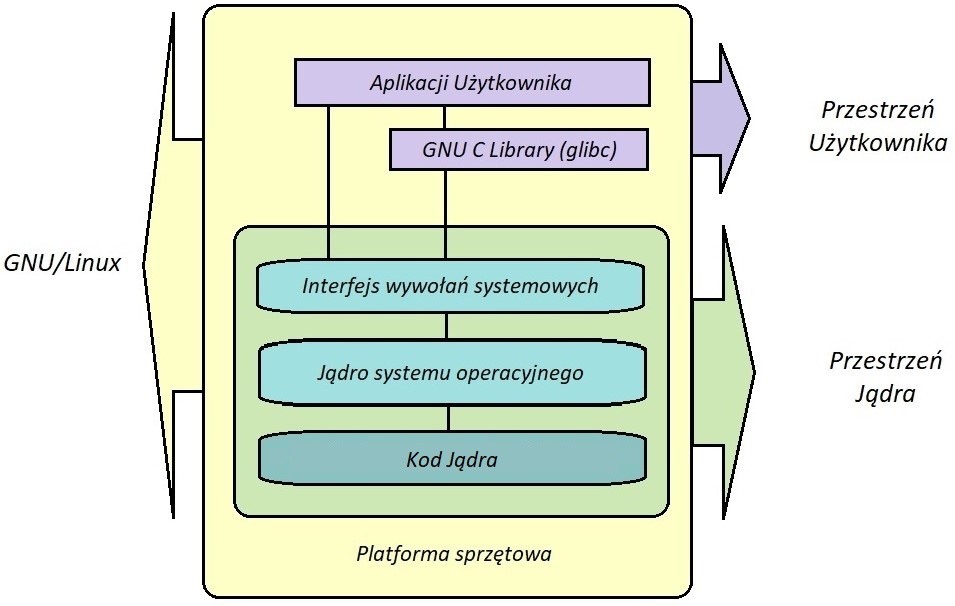
\includegraphics[width=350px]{img/linux-architektura} 
  \captionof{figure}{ \textit{Podstawowa architektura systemu operacyjnego GNU/Linux [4]}} 
\end{center}
\end{minipage}
\begin{minipage}{1\linewidth}
\vspace{0.3cm}
 W pierwszym znajduje się interfejs wywołań systemowych, który implementuje podstawowe funkcje takie jak odczyt i zapis. Na następnym poziomie znajduje się kod jądra, który można zdefiniować jako niezależny od architektury kod. Jest to część kodu systemu operacyjnego, która zawsze rezyduje w pamięci i ułatwia interakcje między komponentami sprzętowymi i programowymi. Na ostatnim poziomie jest kod zależny od architektury,  ten kod jest specyficzny dla procesora i platformy danej architektury.\\ 
\end{minipage}
Funkcje systemu operacyjnego: \\
\begin{adjustwidth}{0.5cm}{0cm}
\begin{minipage}{1\linewidth}
\begin{itemize}
\setlength\itemsep{0.2cm}
    \item[\ding{118}]  Zarządzanie pamięcią — alokuje i dealokuje przestrzeń pamięci dla programów
    \item[\ding{118}]  Zarządzanie procesami — tworzy i usuwa procesy. Zapewnia również mechanizmy synchronizacji i komunikacji między procesami.
    \item[\ding{118}] Zarządzanie plikami — przechowuje, pobiera, nazywa, udostępnia i chroni pliki.
    \item[\ding{118}] Zarządzenie urządzeniami — śledzi wszystkie urządzenia.
    \item[\ding{118}] Zarządzenie urządzeniami we/wy — ukrywanie przed użytkownikiem specyfiki urządzeń sprzętowych.
    \item[\ding{118}] Bezpieczeństwo — chroni dane i informacje systemu przed zagrożeniami.
    \end{itemize}
    \end{minipage}
    \begin{minipage}{1\linewidth}
    \begin{itemize}
    \item[\ding{118}] Połączenie z siecią. 
    \item[\ding{118}] Interpretacja poleceń — interpretuje polecenia wydawane przez zasoby systemowe w celu przetworzenie tych poleceń.
\end{itemize}
\end{minipage}
\end{adjustwidth}
 \begin{minipage}{\linewidth}
\begin{center}
  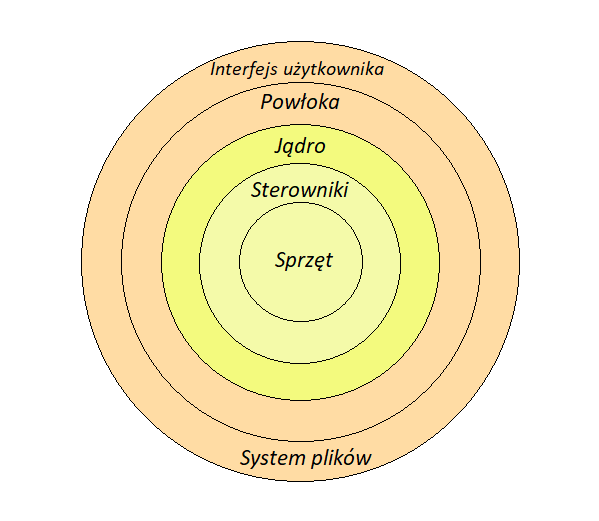
\includegraphics[width=300px]{img/system}
  \captionof{figure}{ \textit{Komponenty systemu operacyjnego. [5]}} 
\end{center}
\end{minipage}
\begin{minipage}{1\linewidth}
\vspace{0.3cm}
Każdy system operacyjny składa się z trzech, podstawowych części: jądra, systemu plików oraz powłoki.
\end{minipage}
\section{Jądro Systemu Operacyjnego}
\begin{minipage}{1\linewidth}
Termin “jądro” oznacza niskopoziomowe oprogramowanie systemowe, które kontroluje wszystkie główne funkcje sprzętu, takie jak zarządzanie pamięcią, procesami itp., niezależnie od tego, czy jest to telefon, laptop, serwer, czy jakikolwiek inny rodzaj komputera. \\ 
\end{minipage}
 \begin{minipage}{\linewidth}
\begin{center}
  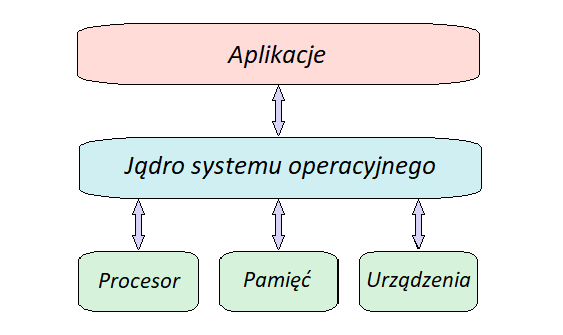
\includegraphics[width=300px]{img/jadro}
  \captionof{figure}{ \textit{Jądro łączące oprogramowanie aplikacji ze sprzętem komputera.}} 
\end{center}
\end{minipage}
\begin{minipage}{1\linewidth}
Zadania jądra systemu operacyjnego: \\
\begin{adjustwidth}{0.5cm}{0cm}
\begin{itemize}
\setlength\itemsep{0.3cm}
    \item[\ding{118}] Obsługa procesów (uruchamianie, zatrzymywanie)
    \item[\ding{118}] Zarządzanie pamięcią
    \item[\ding{118}] Obsługa urządzeń i ich przerwań
    \item[\ding{118}] Zarządza zasobami komputera 
    \item[\ding{118}] Obsługa sieci 
\end{itemize}
\end{adjustwidth}
\vspace{0.3cm}
Jądro Linux jest głównym składnikiem systemu operacyjnego Linux i stanowi podstawowy interfejs między sprzętem komputera a jego procesami. Jądro systemu operacyjnego charakteryzuje się wielozadaniowością i wielowątkowością, dzięki temu jest w stanie realizować kilka różnych zadań w jednym czasie. 
\end{minipage}
\section{Powłoka Systemu Operacyjnego}
\begin{minipage}{1\linewidth}
Powłoka to specjalny program komputerowy, który umożliwia komunikację pomiędzy systemem operacyjnym a użytkownikiem. Powłoki systemu operacyjnego używają interfejsu wiersza poleceń (CLI) lub graficznego interfejsu użytkownika (GUI). Dwie dobrze znane powłoki CLI to PowerShell dla Windows oraz Bash dla Linuksa i macOS. \\ \\
CLI wymaga, od użytkownika znajomość, poleceń i składni oraz zrozumienie pojęć języka skryptowego specyficznego dla powłoki (na przykład bash). Bash jest najczęściej używaną powłoką wiersza poleceń dla systemów operacyjnych opartych na systemie Unix, w tym Linux. \\ \\
GUI pozwala użytkownikom do interakcji z urządzeniami elektronicznymi za pomocą elementów graficznych, takich jak ikony, kursory i przyciski, są czasami wzbogacane dźwiękami lub efektami wizualnymi, takimi jak przezroczystość i cienie. Korzystając z tych obiektów, użytkownik może korzystać z komputera bez znajomości poleceń.
\end{minipage}
\section{System plików}
\begin{minipage}{1\linewidth}
System plików to metoda przechowywania plików, zarządzania plikami, tak aby dostęp do plików i danych w nich zgromadzonych był łatwy dla użytkownika systemu. Bez systemu plików dane umieszczone na nośniku pamięci byłyby jednym dużym zbiorem danych bez możliwości stwierdzenia, gdzie jeden element danych się zatrzymał, a drugi zaczął. Dzięki rozdzieleniu danych na kawałki i nadaniu każdemu kawałkowi nazwy, dane można łatwo wyizolować i zidentyfikować. 
\end{minipage}
\section{Terminal Linux}
\begin{minipage}{1\linewidth}
To interfejs tekstowy, który odbiera polecenia w postaci wierszy tekstu. Jest również znany jako  wiersz poleceń, konsola i wiele innych, jest programem komputerowym przeznaczonym do interpretowania poleceń. Terminal umożliwia jądru i innym procesom wysyłanie danych wyjściowych do użytkownika i otrzymywanie danych wejściowych od użytkownika. Użytkownik zazwyczaj wprowadza tekst za pomocą klawiatury komputera i odczytuje tekst wyjściowy na monitorze. \\ \\
Jest to tylko jedno z wielu narzędzi udostępnianych użytkownikom Linuksa w celu wykonania
dowolnego zadania na przykład instalować różne rzeczy, przenosić pliki, zmieniać uprawnienia do folderów lub plików, zmieniać ustawienia parametrów środowiska, wywoływanie plików wykonywalnych i dostarczenie im informacji o tym, jakie działania mają wykonać, konfigurować pewne aspekty systemu w zależności od dystrybucji, takie jak połączenie internetowe lub sterowniki karty graficznej.
\end{minipage}
\begin{minipage}{1\linewidth}
Polecenie, systemu operacyjnego Linux, są często programami uruchamianymi z wiersza poleceń. Jest to specjalne słowo kluczowe, którego można użyć w terminalu, aby wymusić wykonanie pewnej akcji. Większość poleceń to małe aplikację, które są instalowane z resztą systemu operacyjnego. Zwykle są przechowywane w mało znanych katalogach, takich jak /bin, /sbin, /usr/bin, oraz /usr/sbin, dzięki zmiennej środowiskowej PATH terminal wie, gdzie je znaleźć. Inne polecenia są wbudowane w terminal. \\
\end{minipage}
 \begin{minipage}{\linewidth}
\begin{center}
  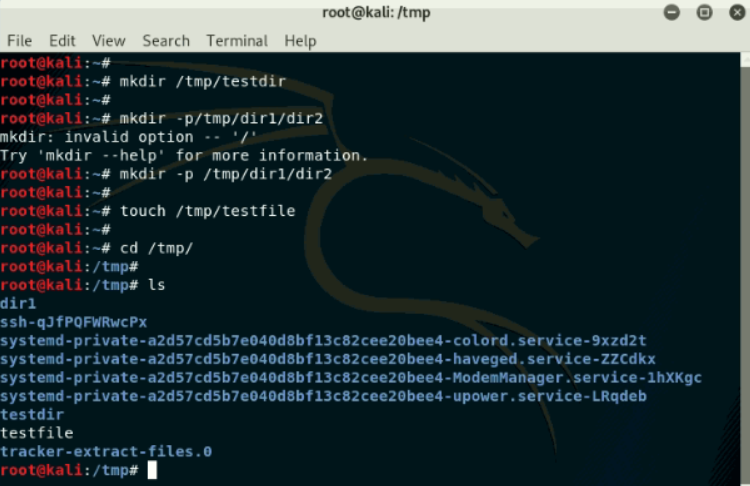
\includegraphics[width=300px]{img/terminal}
  \captionof{figure}{ \textit{Przykładowe okno terminala}} 
\end{center}
\end{minipage}
\chapter{Wykorzystane narzędzia}
\section{Frontend}
\subsection{HTML}
\begin{minipage}{1\linewidth}
HTML lub HyperText Markup Language to standardowy język znaczników do tworzenia stron internetowych. Znaczniki HTML otoczone są nawiasami kątowymi, mogą też zawierać w sobie podrzędne znaczniki. Znaczniki umożliwiają dodanie takich elementów jak: obrazy, formularze interaktywne, listy, tabele i wiele innych. Przeglądarki nie wyświetlają znaczników, tylko używają ich do interpretacji zawartości strony. HTML może osadzać programy napisane w języku skryptowym, takim jak JavaScript, co wpływa na zachowanie i zawartość stron internetowych. Warto zauważyć, że HTML nie jest uważany za język programowania, ponieważ nie może tworzyć dynamicznych funkcji. 
\end{minipage}
\subsection{CSS}
\begin{minipage}{1\linewidth}
CSS jest to kaskadowy arkusz stylów, który służy do nadania odpowiedniego wyglądu stronie internetowej. Jest zwykle używany z HTML do zmiany stylu stron internetowych i interfejsów użytkownika. Za pomocą CSS możesz kontrolować kolor tekstu, styl czcionek, odstępy między akapitami, rozmiar i układ kolumn, używane obrazy lub kolory tła, a także wiele innych efektów. \\
\end{minipage}
\begin{center}
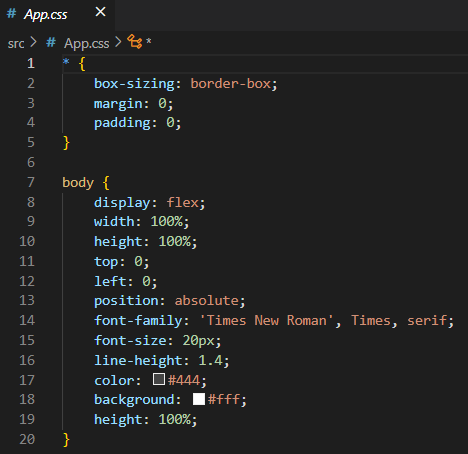
\includegraphics[width=230px]{img/css}
\begin{lstlisting}[escapeinside=``,caption={Przykładowe użycie CSS w projekcie}]
`\vspace{-1.5cm}`
\end{lstlisting}
\end{center}
\vspace{0.1cm}
\subsection{JavaScript}
\begin{minipage}{1\linewidth}
JavaScript  jest dynamicznym językiem programowania, który często jest używany do tworzenia bardziej dynamicznych interakcji podczas tworzenia stron internetowych, aplikacji, serwerów, a nawet gier. Jako język skryptowy po stronie klienta, jest to jedna z podstawowych technologii sieci WWW. Programiści zazwyczaj używają JavaScript razem z HTML i CSS, ponieważ JavaScript oferuje rozszerzone możliwości, których oni nie mogą zapewnić. JavaScript sprawia, że strony internetowe stają się bardziej interaktywne na wiele sposobów na przykład wyświetlanie animacji, tworzenie funkcjonalnych menu rozwijanych, powiększanie i pomniejszanie obrazów stron internetowych, a nawet zmienianie kolorów przycisków, gdy użytkownik najedzie na nie myszą. 
\end{minipage}
\subsection{React}
\begin{minipage}{1\linewidth}
React jest darmową biblioteką JavaScript do budowania interfejsów użytkownika w oparciu o komponenty UI. React może być używany do tworzenia aplikacji jednostronicowych , mobilnych lub renderowanych na serwerze z frameworkami takimi jak Next.js . Tworzenie aplikacji React zwykle wymaga użycia dodatkowych bibliotek do routingu, a także pewnych funkcji po stronie klienta. \\
\end{minipage}
\begin{center}
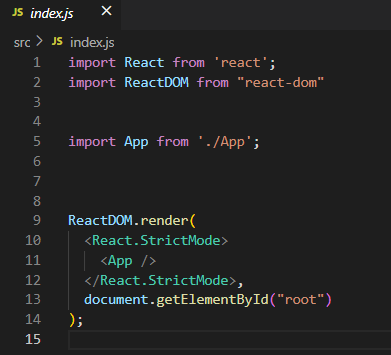
\includegraphics[width=230px]{img/react}
\begin{lstlisting}[escapeinside=``,caption={Przykładowe użycie Reacta w projekcie}]
`\vspace{-1cm}`
\end{lstlisting}
\end{center}
\begin{minipage}{1\linewidth}
React używa JSX do tworzenia "elementów". JSX jest rozszerzeniem składni JavaScript, które używa Babel do konwersji tekstu podobnego do HTML w plikach JavaScript na obiekty JavaScript. React nie wymaga korzystania z JSX , ale większość programistów uważa, że jest to bardziej przyjazne dla użytkownika w kodzie JavaScript.
\end{minipage}
\section{Backend}
\subsection{Java}
\begin{minipage}{1\linewidth}
Java to oparty na klasach, obiektowy  język programowania, który  jest popularny w prawie wszystkich branżach. 
Ważną rzeczą w Javie, która odróżnia ją od wielu innych technologii, jest to, że została zaprojektowana w taki sposób, aby kod napisany w Javie mógł być uruchamiany na dowolnym systemie, na którym może działać wirtualna maszyna Javy (JVM). 
\end{minipage}
\subsection{Maven}
\begin{minipage}{1\linewidth}
Maven to narzędzie służące do zautomatyzowania budowania projektów napisanych w Javie.
Bezproblemowo obsługuje kompilację, dystrybucję, dokumentację i inne zadania.
\end{minipage}
\begin{minipage}{1\linewidth}
Podstawowym celem Mavena jest zapewnienie deweloperom następujących składników:
\begin{itemize}
    \item Kompleksowy model projektów, który można ponownie wykorzystać, konserwować i łatwiej zrozumieć.
    \item Wtyczki lub narzędzia, które współdziałają z tym deklaratywnym modelem.
\end{itemize} 
Struktura i zawartość projektu Maven są deklarowane w pliku pom.xml, zwanym Project Object Model (POM), który jest podstawową jednostką całego systemu Maven.
\vspace{0.2cm}
\end{minipage}
\begin{center}
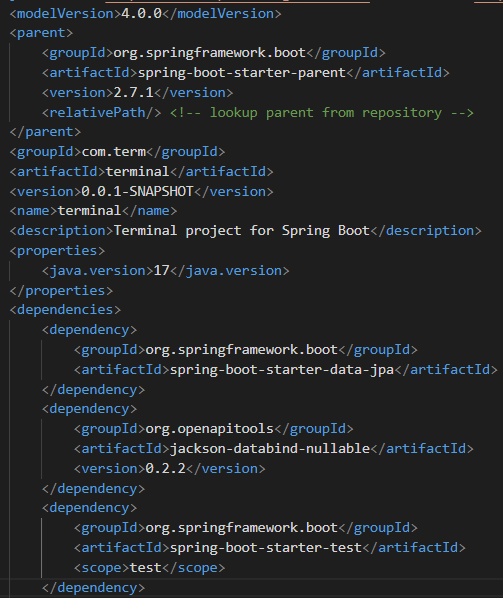
\includegraphics[width=200px]{img/pom}
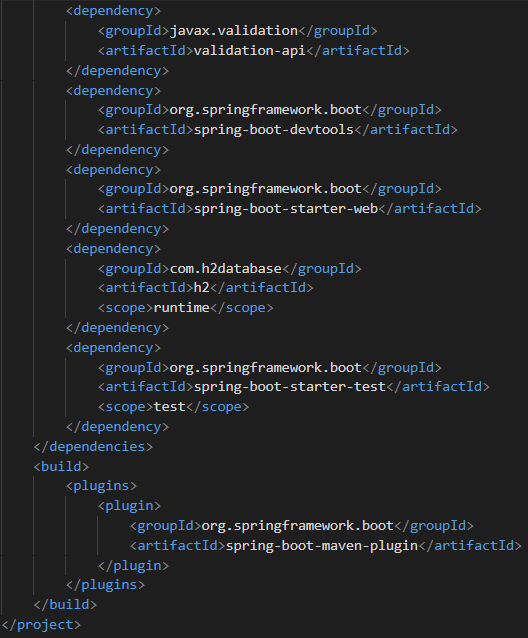
\includegraphics[width=200px]{img/pom1} 
\begin{lstlisting}[escapeinside=``,caption={Przykładowe użycie pliku pom.xml w projekcie}]
`\vspace{-1.5cm}`
\end{lstlisting}
\end{center}
\subsection{Spring Boot}
\begin{minipage}{1\linewidth}
Spring Boot jest frameworkiem, który pozwala tworzyć zaawansowane aplikacje przy stosunkowo małej ilości kodu oraz stanowi bibliotekę szablonów, która dostarcza narzędzia ułatwiające pracę programisty. Jeśli chcesz stworzyć aplikację webową wystarczy użyć odpowiedniej zależności (Maven dependency) reprezentującej szablon startowy do budowy aplikacji web, a wszystkie wymagane zależności zostaną automatycznie dodane do projektu.
Własności aplikacji Spring Boot określane są w pliku application.properties. 
\vspace{0.2cm}
\end{minipage}
\begin{center}
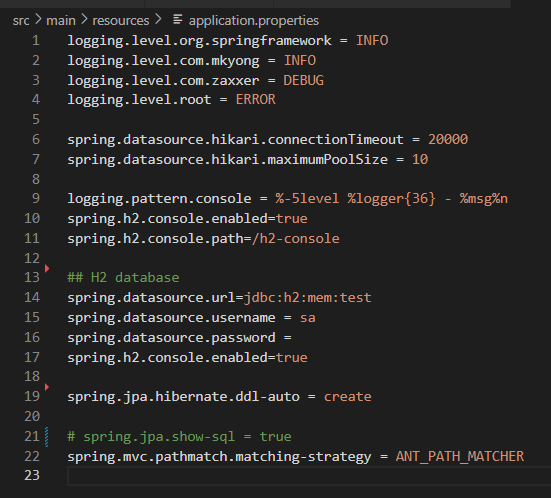
\includegraphics[width=200px]{img/properties} 
\begin{lstlisting}[escapeinside=``,caption={Przykładowe użycie pliku application.properties w projekcie}]
`\vspace{-1.5cm}`
\end{lstlisting}
\end{center}
\subsection{Hibernate}
\begin{minipage}{1\linewidth}
Hibernate to narzędzie do Javy, które służy do mapowania obiektowo-relacyjnego. Podstawową cechą Hibernate jest mapowanie z klas Java na tabele bazy danych oraz mapowanie z typów danych Java na typy danych SQL . Jest dobrze znany ze swojej stabilności i jakości, czego dowodem jest akceptacja i użytkowanie przez dziesiątki tysięcy programistów Java.
\end{minipage}
\subsection{Baza danych H2}
\begin{minipage}{1\linewidth}
H2 to baza danych Java SQL o otwartym kodzie źródłowym. Może działać zarówno w trybie klient-serwer, jak i wbudowanym. Baza danych jest przechowywana w pamięci operacyjnej z tego powodu jest używana w środowiskach deweloperskich i testowych. Korzystamy z takiej bazy, gdy nie musimy utrwalać danych, po ponownym uruchomieniu aplikacji wszystkie przechowywane dane zostaną utracone. Dodatkowym atutem bazy H2 jest wbudowana w przeglądarkę konsola oraz mały rozmiar. \\
\end{minipage}
 \begin{minipage}{\linewidth}
\begin{center}
  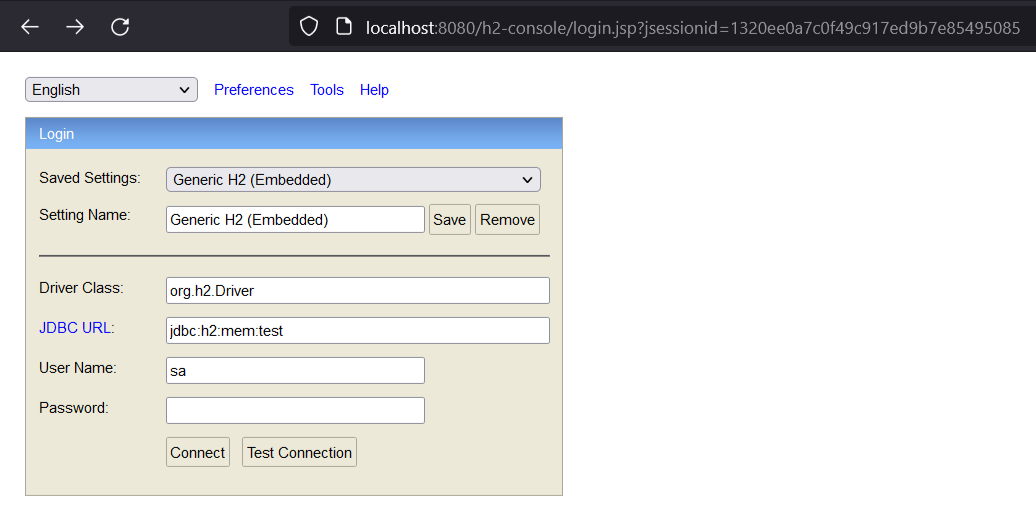
\includegraphics[width=400px]{img/h2_console}
  \captionof{figure}{ \textit{Przykładowe użycie konsoli bazy danych H2 w projekcie}} 
\end{center}
\end{minipage}
 \begin{minipage}{\linewidth}
\vspace{0.5cm}
\begin{center}
  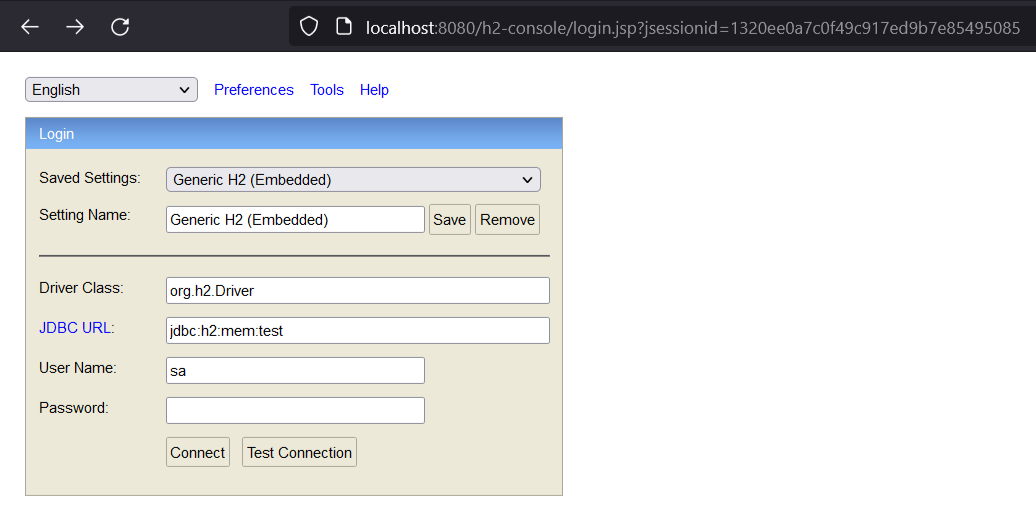
\includegraphics[width=400px]{img/h2_console} 
  \captionof{figure}{ \textit{Przykładowe użycie konsoli bazy danych H2 w projekcie}} 
\end{center}
\end{minipage}
\chapter{Projekt}
\section{Założenia}
\begin{minipage}{1\linewidth}
Głównym celem pracy jest utworzenie dydaktycznej aplikacji imitującej zachowanie wiersza poleceń, która będzie służyć do wspomagania nauki terminala Linuxa. \\ \\
Główne założenia to:
\begin{itemize}
\setlength\itemsep{0.3cm}
    \item[\ding{118}] Napisanie aplikacji webowej, która będzie  umożliwiała naukę terminala Linux przez praktykę. Użytkownicy będą mogli wpisać w terminalu dowolne dozwolone polecenie i zobaczyć jego działanie w swojej przeglądarce  bez konieczności instalowania Linuxa lub uruchamiania go na wirtualnej maszynie. 
    \item[\ding{118}] W aplikacji będą zawarte podstawowe polecenia terminala Linux, takie jak: ls, cd, cp, mv, cat, rm, mkdir, rmdir, touch, nano, man. Wprowadzając polecenie ‘man’ w imitacji terminala, zostaną wyświetlone polecenia które można używać w danym terminalu.
    \item[\ding{118}] Użytkownicy będą mogli utrwalać swoją wiedzę rozwiązując quiz. 
    \item[\ding{118}] Przed przejściem do rozwiązania wybranego quizu użytkownik będzie mógł przeczytać krótki opis poleceń zawartych w danym quizie.
    \item[\ding{118}] Podczas rozwiązywania quizu użytkownicy będą mogli sprawdzać swoje odpowiedzi wpisując odpowiednie polecenia w terminalu.
    \item[\ding{118}] Dodatkową funkcjonalnością aplikacji będzie możliwość pozostawiania przez użytkowników pytań związanych z terminalem Linux. Użytkownicy będą mogli również zostawiać swoje komentarze pod wybranymi pytaniami.
\end{itemize}
\end{minipage}
 \begin{minipage}{\linewidth}
\begin{center}
  
\includegraphics[width=200px]{project/logo.png} 
  \captionof{figure}{ \textit{Logo aplikacji TermTrain}} 
\end{center}
\end{minipage}
\section{Przypadki użycia}
\begin{minipage}{1\linewidth}
W ramach projektu aplikacji będącej tematem niniejszej pracy, w tym rozdziale w celu dokładniejszego opisu wymagań aplikacji, wykonane zostały opisy przypadków użycia, jak również graficzne ich przedstawienie z użyciem języka UML w postaci diagramu (Rys. 3.2).
\end{minipage}
\begin{adjustwidth}{-2cm}{-2cm}
 \begin{minipage}{\linewidth}
\vspace{0.2cm}
\begin{center}
  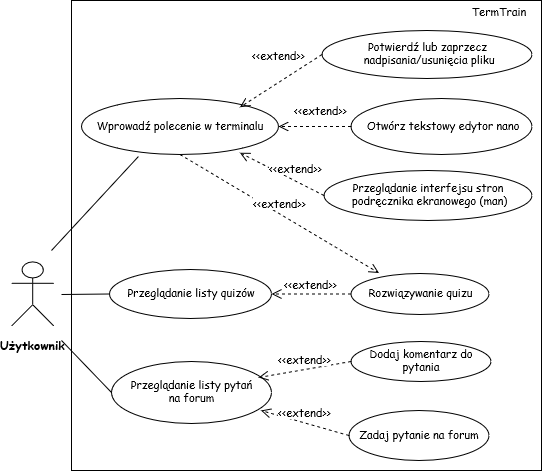
\includegraphics[width=350px]{img/diagram}
  \captionof{figure}{ \textit{Diagram przypadków użycia}} 
\end{center}
\end{minipage}
\end{adjustwidth}
\subsection{Wprowadź polecenie w terminalu}
\begin{minipage}{1\linewidth}
\textbf{Krótki opis:} Przypadek użycia umożliwia użytkowniku wprowadzenie w aplikacji, imitującej zachowanie wiersza poleceń, komendę w celu wykonania pewnej czynności. \\ \\
\textbf{Warunek początkowy:} Jest otwarta strona główna. \\ \\
\textbf{Zdarzenie inicjujące:} Przypadek użycia zaczyna się, gdy użytkownik wybierze w głównym menu zakładkę Terminal. \\ \\
\textbf{Główny scenariusz:} 
\begin{enumerate}
\setlength\itemsep{0.2cm}
    \item Użytkownik wybiera zakładkę Terminal.
    \item Aplikacja wyświetla imitacje wiersza poleceń.
    \item Użytkownik wprowadza w terminalu pewne polecenie(np. cd, ls, cat itp.).
    \item Aplikacja wykonuje pewną czynność w zależności od wybranego polecenia.
\end{enumerate}
\end{minipage}
\subsection{Potwierdź lub zaprzecz nadpisanie/usunięcie pliku}
\begin{minipage}{1\linewidth}
\textbf{Krótki opis:} Przypadek użycia umożliwia użytkowniku usunięcie lub nadpisanie plików po wprowadzeniu w terminalu odpowiednich poleceń.
\end{minipage}
\begin{minipage}{1\linewidth}
\textbf{Warunek początkowy:} Jest otwarty ekran przedstawiający imitację terminala Linux. \\ \\
\textbf{Zdarzenie inicjujące:} Przypadek użycia zaczyna się, gdy  użytkownik wprowadza jedne z trzech poleceń, takich jak cp, mv lub rm, z flagą -i. \\ \\
\textbf{Główny scenariusz:} 
\begin{enumerate}
\setlength\itemsep{0.2cm}
    \item Użytkownik wprowadza w terminalu jedno z poleceń używając flagę -i.
    \item Aplikacja wyświetla komunikat, w którym użytkownik jest pytany o potwierdzenie lub zaprzeczenia nadpisania/usunięcia pliku.
    \item Użytkownik wprowadza w terminale odpowiedź( yes lub no).
    \item Aplikacja wykonuje pewną czynność w zależności od wybranego polecenia.
\end{enumerate}
\end{minipage}
\subsection{Otwórz tekstowy edytor nano}
\begin{minipage}{1\linewidth}
\textbf{Krótki opis:} Przypadek użycia umożliwia użytkowniku otworzenie tekstowego edytora nano. W edytorze użytkownik będzie mógł wprowadzić jakiś tekst lub edytować już istniejący i zapisać zmiany do danego pliku używając skrótu Ctrl+q żeby wyjść z trybu edytowania trzeba użyć skrótu Ctrl+x. \\ \\
\textbf{Warunek początkowy:} Jest otwarty ekran przedstawiający imitację terminala Linux. \\ \\
\textbf{Zdarzenie inicjujące:} Przypadek użycia zaczyna się, gdy użytkownik wprowadza polecenie "nano nazwa\_pliku". \\ \\
\textbf{Główny scenariusz:} 
\begin{enumerate}
\setlength\itemsep{0.2cm}
    \item Użytkownik wprowadza w terminalu polecenie "nano nazwa\_pliku".
    \item Aplikacja wyświetla okno do wprowadzenia tekstu.
    \item Użytkownik wprowadza jakiś tekst lub zostawia puste pole. 
    \item Użytkownik używa skrótu Gtrl+q, aby zapisać wprowadzony tekst.
    \item Przejdź do punktu 3, do póki użytkownik nie użyje skrótu Gtrl+x, aby wyjść z edytora nano. 
    \item Aplikacja zamyka okno do wprowadzenia tekstu i wraca do wiersza poleceń.
\end{enumerate}
\end{minipage}
\subsection{Przeglądanie interfejsu stron podręcznika ekranowego(man)}
\begin{minipage}{1\linewidth}
\textbf{Krótki opis:} Przypadek użycia umożliwia użytkowniku przeglądanie interfejsu stron podręcznika ekranowego(man). Aby zamknąć stronę man trzeba nacisnąć na "q". \\ \\
\textbf{Warunek początkowy:} Jest otwarty ekran przedstawiający imitację terminala Linux.\\ \\
\textbf{Zdarzenie inicjujące:} Przypadek użycia zaczyna się, gdy użytkownik wprowadza polecenie "man".
\textbf{Główny scenariusz:} 
\begin{enumerate}
\setlength\itemsep{0.2cm}
    \item Użytkownik wprowadza w terminalu polecenie "man".
    \item Aplikacja wyświetla okno, w którym wyświetla stronę man.
    \item Użytkownik przegląda stronę.
    \item Użytkownik naciska na "q", aby zamknąć stronę man. 
    \end{enumerate}
    \end{minipage}
   \begin{minipage}{1\linewidth}
   \begin{enumerate}
    \item Aplikacja zamyka okno wyświetlające interfejs stron podręcznika ekranowego i wraca do wiersza poleceń.
\end{enumerate}
\end{minipage}
\subsection{Przeglądanie listy quizów}
\begin{minipage}{1\linewidth}
\textbf{Krótki opis:} Przypadek użycia umożliwia użytkowniku przeglądanie listy quizów. Użytkownik także może zobaczyć swój wynik po rozwiązaniu quizu. Może także wyświetlić informacje o określonych poleceniach, które są wykorzystywane w quizie, oraz przejść do rozwiązywania quizu.  \\ \\
\textbf{Warunek początkowy:} Jest otwarty jakikolwiek ekran z głównym menu w którym jest zakładka Quiz. \\ \\
\textbf{Zdarzenie inicjujące:} Przypadek użycia zaczyna się, gdy użytkownik wybierze w głównym menu zakładkę Quiz. \\ \\
\textbf{Główny scenariusz:} 
\begin{enumerate}
\setlength\itemsep{0.2cm}
    \item Aplikacja wyświetla listę quizów.
    \item Użytkownik wybiera opcję "rozwiąż quiz" wybranego quizu
    \item Aplikacja wyświetla po lewej stronie imitacje wiersza poleceń, a po prawej quiz. \\
\end{enumerate}
\textbf{Alternatywny scenariusz:} 
\begin{enumerate}
\setlength\itemsep{0.2cm}
    \item Aplikacja wyświetla listę quizów.
    \item Użytkownik wybiera opcję "teoria" wybranego quizu.
    \item Aplikacja wyświetla okno z informacją o poleceniach znających się w danym quizie.
    \item Użytkownik zamyka okno.
    \item Przejście do punktu 1 głównego scenariusza.
\end{enumerate}
\end{minipage}
\subsection{Rozwiązywanie quizu}
\begin{minipage}{1\linewidth}
\textbf{Krótki opis:} Przypadek użycia umożliwia użytkowniku przejście do rozwiązywanie wybranego quizu. Pod czas rozwiązywania quizu użytkownik ma możliwość sprawdzenie poprawnej odpowiedzi w imitacji terminala Linux. Po zakończeniu rozwiązywania quizu jest wyświetlany wynik. \\ \\
\textbf{Warunek początkowy:} Jest otwarty ekran przedstawiający listę quizów.\\ \\
\textbf{Zdarzenie inicjujące:} Przypadek użycia zaczyna się, gdy użytkownik wybiera w opcję "Rozwiąż quiz" wybranego quizu. \\
\textbf{Główny scenariusz:} 
\begin{enumerate}
\setlength\itemsep{0.2cm}
    \item Użytkownik zaznacza odpowiedź.
    \item Użytkownik wybiera przycisk "next".
    \item Aplikacja wyświetla następne pytanie
    \item Przejście do punktu 1, dopóki nie zostanie wyświetlony wynik.
    \item Aplikacja wyświetla wynik.
\end{enumerate}
\end{minipage}
\begin{minipage}{1\linewidth}
\textbf{Alternatywny scenariusz:} 
\begin{enumerate}
\setlength\itemsep{0.2cm}
    \item Użytkownik zaznacza odpowiedź.
    \item Użytkownik sprawdza odpowiedź w terminalu.
    \item Aplikacja wykonuje pewną czynność w zależności od wprowadzonego polecenia.
    \item Użytkownik wybiera przycisk "next".
    \item Aplikacja wyświetla następne pytanie.
    \item Przejście do punktu 1, dopóki nie zostanie wyświetlony wynik.
    \item Aplikacja wyświetla wynik.
\end{enumerate}
\end{minipage}
\subsection{Przeglądanie listy pytań na forum}
\begin{minipage}{1\linewidth}
\textbf{Krótki opis:} Przypadek użycia umożliwia użytkowniku przeglądanie listy pytań na forum. Użytkownik widzi pytania umieszczone na forum, może dodać komentarze pod wybranym pytaniem. Także może zostawić swoje pytanie.   \\ \\
\textbf{Warunek początkowy:} Jest otwarty jakikolwiek ekran z głównym menu w którym jest zakładka Forum \\ \\
\textbf{Zdarzenie inicjujące:} Przypadek użycia zaczyna się, gdy użytkownik wybierze w głównym menu zakładkę Forum. \\ \\
\textbf{Główny scenariusz:} 
\begin{enumerate}
\setlength\itemsep{0.2cm}
    \item Aplikacja wyświetla pytań na forum.
    \item Użytkownik wybiera interesujące go pytanie.
    \item Aplikacja wyświetla szczegóły dotyczące danego pytania oraz miejsce na zostawiania komentarzy.
\end{enumerate}
\end{minipage}
\subsection{Zadaj pytanie na forum}
\begin{minipage}{1\linewidth}
\textbf{Krótki opis:} Przypadek użycia umożliwia użytkowniku dodanie pytania do listy pytań na forum.   \\ \\
\textbf{Warunek początkowy:} Jest otwarty ekran przedstawiający listę pytań na forum.  \\ \\
\textbf{Zdarzenie inicjujące:} Przypadek użycia zaczyna się, gdy użytkownik kliknie na przycisk plusa. 
\textbf{Główny scenariusz:} 
\begin{enumerate}
\setlength\itemsep{0.2cm}
    \item Użytkownik wybiera przycisk ze znakiem plusa. 
    \item Aplikacja wyświetla okno z edytowalnymi przez użytkownika polami przeznaczonymi na nazwę i opis pytania oraz przyciskiem służącym do zapisania pytania i przyciskiem służącym do zamknięcia okna.
    \item Użytkownik zapisuje pytanie.
    \item Aplikacja dodaje pytanie do listy pytań.
    \item Użytkownik wybiera przycisk służący do wyjścia.
    \item Aplikacja zamyka okno i wraca do listy pytań..
\end{enumerate}
\end{minipage}
\begin{minipage}{1\linewidth}
\textbf{Alternatywny scenariusz:} 
\begin{enumerate}
\setlength\itemsep{0.2cm}
    \item Użytkownik wybiera przycisk ze znakiem plusa.
    \item Aplikacja wyświetla okno z edytowalnymi przez użytkownika polami przeznaczonymi na nazwę i opis pytania oraz przyciskiem służącym do zapisania pytania i przyciskiem służącym do zamknięcia okna.
    \item Użytkownik zrezygnował z dodania pytania i wybiera przycisk służący do zamknięcia okna.
    \item Aplikacja zamyka okno i wraca do listy pytań.
\end{enumerate}
\end{minipage}
\subsection{Dodaj komentarz do pytania}
\begin{minipage}{1\linewidth}
\textbf{Krótki opis:} Przypadek użycia umożliwia użytkowniku zostawianie komentarzy pod wybranymi pytaniami. Użytkownik też może polubić wybrany komentarz.\\ \\
\textbf{Warunek początkowy:} Jest otwarty ekran przedstawiający szczegóły dotyczące konkretnego pytania.\\ \\
\textbf{Zdarzenie inicjujące:} Przypadek użycia zaczyna się, gdy użytkownik wybierze w głównym menu zakładkę Forum. \\ \\
\textbf{Główny scenariusz:} 
\begin{enumerate}
\setlength\itemsep{0.2cm}
    \item Aplikacja wyświetla szczegóły dotyczące danego pytania oraz miejsce na zostawiania pytań. 
    \item Użytkownik zostawia swój komentarz.
    \item Aplikacja dodaje komentarz do listy komentarzy.
\end{enumerate}
\end{minipage}
\section{Baza danych}
\begin{minipage}{1\linewidth}
Baza danych wykorzystana w projekcie ma formę siedmiu tabel \textit{quiz\_table, question\_table, answer\_table, account\_table, forum\_table, comment\_table i listOfResult\_table} (Rys. 3.3).
\vspace{0.3cm}
\end{minipage}
 \begin{minipage}{\linewidth}
\begin{center}
  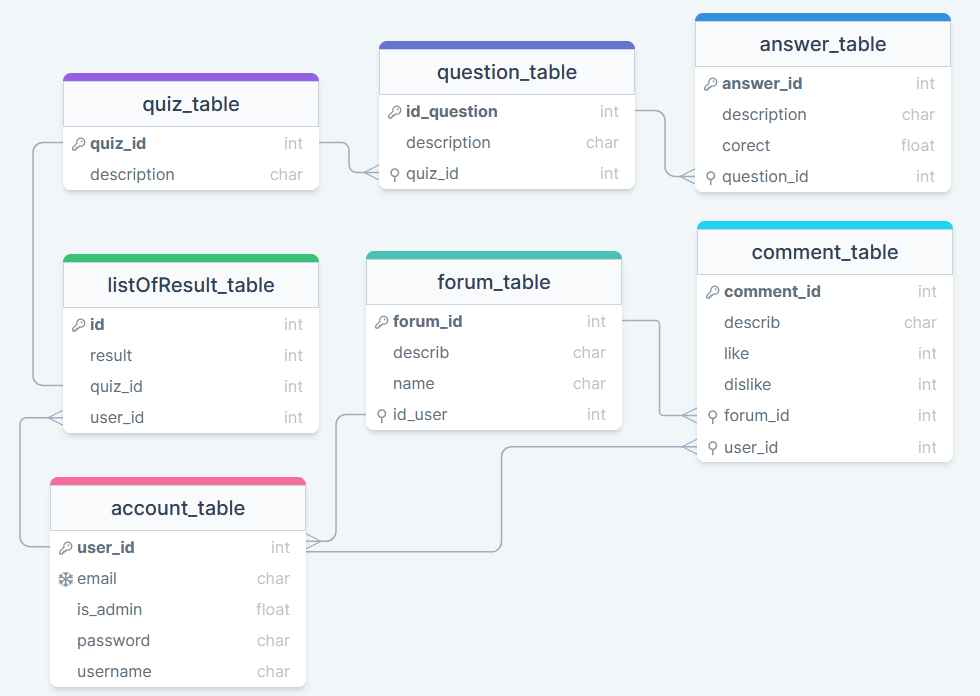
\includegraphics[width=320px]{img/database.png}
  \captionof{figure}{ \textit{Diagram bazy danych}} 
\end{center}
\end{minipage}
\begin{minipage}{1\linewidth}
\vspace{0.3cm}
Tabela account\_table przechowuje podstawowe dane o użytkownikach potrzebne do zalogowania takie jak hasło, nazwa użytkownika oraz email. Tabela  quiz\_table przechowuje dane potrzebne do wyświetlenia listy quizów. Tabela question\_table przechowuje dane potrzebne do wyświetlania pytań w konkretnym quizie. Tabela answer\_table przechowuje dane potrzebne do wyświetlenia opcji odpowiedzi w konkretnym pytaniu quizu. Natomiast tabela listOfResults\_table przechowuje wyniki uzyskane przez użytkownika po przejściu konkretnego quizu, dane są aktualizowane po ponownym rozwiązaniu quizu. Tabela forum\_table przechowuje dane potrzebne do wyświetlenia listy putan na forum. Tabela comment\_table przechowuje dane potrzebne do wyświetlenia listy komentarzy konkretnego pytania. 
\end{minipage}
\section{Implementacja}
\begin{minipage}{1\linewidth}
W tym rozdziale zostały omówione główne komponenty z których jest zbudowana  fontendowa część aplikacji. Na początku omówione zostanie drzewo katalogów, później metoda render() w komponentach Terminal oraz Commands, na koniec zostanie opisany routing oraz komponent Nano. 
\end{minipage}
\subsection{Drzewo katalogów części frontendowej aplikacji}
\begin{minipage}{1\linewidth}
Wszystkie komponenty aplikacji  znajdują się w katalogu src(Rys. 3.4).\\
\end{minipage}
 \begin{minipage}{\linewidth}
\begin{center}
  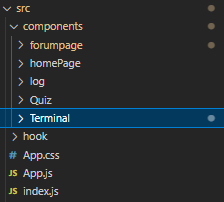
\includegraphics[width=150px]{code/drzewo.png}
  \captionof{figure}{ \textit{Drzewo katalogów wykorzystane w części frontendowej aplikacji}} 
\end{center}
\end{minipage}
\begin{minipage}{1\linewidth}
\vspace{0.3cm}
Zaczynając od pliku index.js, który zawiera logikę renderowania komponentu App.js. Głównym celem pliku index.js jest zaimportowanie wszystkich niezbędnych do skonfigurowania aplikacji elementów oraz uruchomienie jej. Plik App.js jest głównym komponentem aplikacji React. Przechodząc do katalogu components który składa się z pięciu katalogów podstawowych komponentów, \textit{forumpage, homepage, log, Quiz i Terminal}. W katalogu forumpage znajdują się komponenty odpowiadające za zachowanie zakładki Forum, dodawania nowych pytań, przeglądanie szczegółów konkretnego pytania oraz dodawanie komentarzy. Komponenty katalogu homepage odpowiadają za zachowanie strony głównej aplikacji. W katalogu log znajdują się komponenty odpowiadające za zachowanie strony logowania oraz rejestracji. Komponenty katalogu Quiz odpowiadają za zachowanie widoku listy quizów, widoku strony podczas rozwiązywania konkretnego quizu oraz widoku służącego do dodawania i usuwania quizów. 
\vspace{-0.1cm}
\end{minipage}
\begin{multicols}{2}
\begin{minipage}{\linewidth}
\begin{center}
  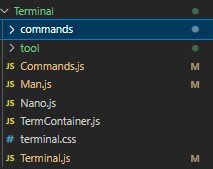
\includegraphics[width=130px]{code/terminal.png}
  \captionof{figure}{ \textit{Zawartość katalogu Terminal}} 
\end{center}
\end{minipage}
\begin{minipage}{\linewidth}
\begin{center}
  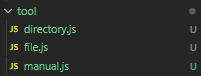
\includegraphics[width=130px]{code/tool.png}
  \captionof{figure}{ \textit{Pliki w katalogu tool}} 
\end{center}
\end{minipage}
\end{multicols}
\begin{adjustwidth}{0cm}{0cm}
\begin{minipage}{\linewidth}
W katalogu Terminal(Rys. 3.5) znajdują się komponenty odpowiadające za zachowania okna imitującego zachowanie terminala Linux. Katalog commands(Rys. 3.7) zawiera pliki z kodem symulujący zachowanie odpowiednich poleceń terminala, nazwy plików odpowiadają nazwom konkretnych poleceń. Pliki file.js oraz directory.js z katalogu tool(Rys. 3.6) odpowiadają za przechowywania podstawowych informacji o plikach i katalogach, a w pliku manual.js są przechowywane strony man.
\end{minipage}
\end{adjustwidth}
\subsection{Komponenty odpowiedzialne za działanie terminala}
\begin{minipage}{1\linewidth}
Komponent Terminal odpowiada za podstawowe funkcje wykonywane w oknie imitującym zachowanie terminala Linux. Podczas renderowania(Listing 3.1) zwracane są linijki kodu odpowiadające za wyświetlenie wiersza poleceń w oknie terminala w odpowiednich kolorach oraz z odpowiednimi danymi. Jednocześnie jest renderowany komponent Commands, który jako argumenty otrzymuje zmienne oraz funkcje znajdujące się w komponencie Terminal. W zależności od  tego jaka komenda została wprowadzona w imitacji  wiersza poleceń w komponencie Terminal wywołują się odpowiednie funkcję, a na wyjściu jest wyprowadzany ich wynik działania. Jeżeli użytkownik wprowadzi polecenie "nano" lub "man" to dodatkowo będzie renderowany jeden z dwóch komponentów Nano lub Man.
\end{minipage}
\vspace{0.3cm}
\begin{center}
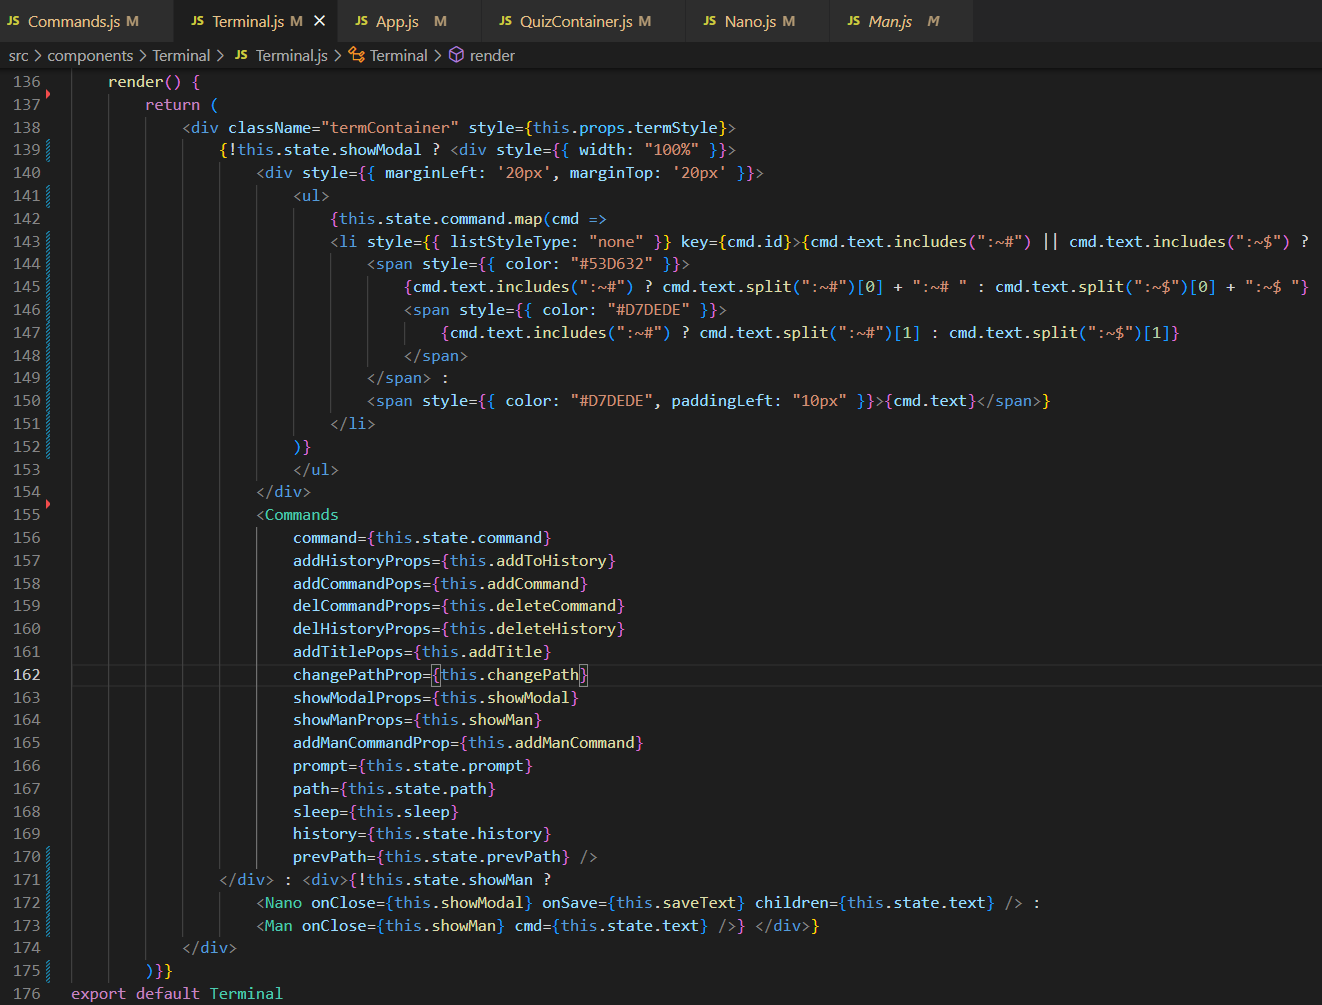
\includegraphics[width=400px]{code/term_code.png} 
\begin{lstlisting}[escapeinside=``,caption={Renderowanie w komponencie Terminal}]
`\vspace{-1.3cm}`
\end{lstlisting}
\end{center}
\vspace{0.3cm}
\begin{minipage}{1\linewidth}
W komponencie Commands wywoływane są funkcje, w które odpowiadają za poprawne działanie poszczególnych poleceń. W danym komponencie podczas renderowania(Listing 3.2) sprawdzane są sygnały wejściowe aplikacji, takie jak  naciśnięcie przez użytkownika którejś z klawiszy.
Jeżeli użytkownik naciśnie na klawisze strzałek góra lub dół, to w zależności od wybranej klawiszy zostanie przewijana historia wprowadzonych poleceń. Po naciśnięciu klawiszy Enter sprawdzane są wprowadzone przez użytkownika polecenie, jeśli dana komenda nie została zaprogramowana, to na wyjściu zostanie wyświetlona informacja o nie istniejącym poleceniu, jeśli jednak ta komenda została zaprogramowana, to na wyjściu zostanie wyświetlony wynik działania konkretnego polecenia. Gdyby użytkownik chciał skorzystać z poleceń rm, mv lub cp z flagą "-i", to na wyjściu zostanie zapytany o pozwolenie nadpisania istniejącego już pliku.
\end{minipage}
\begin{center}
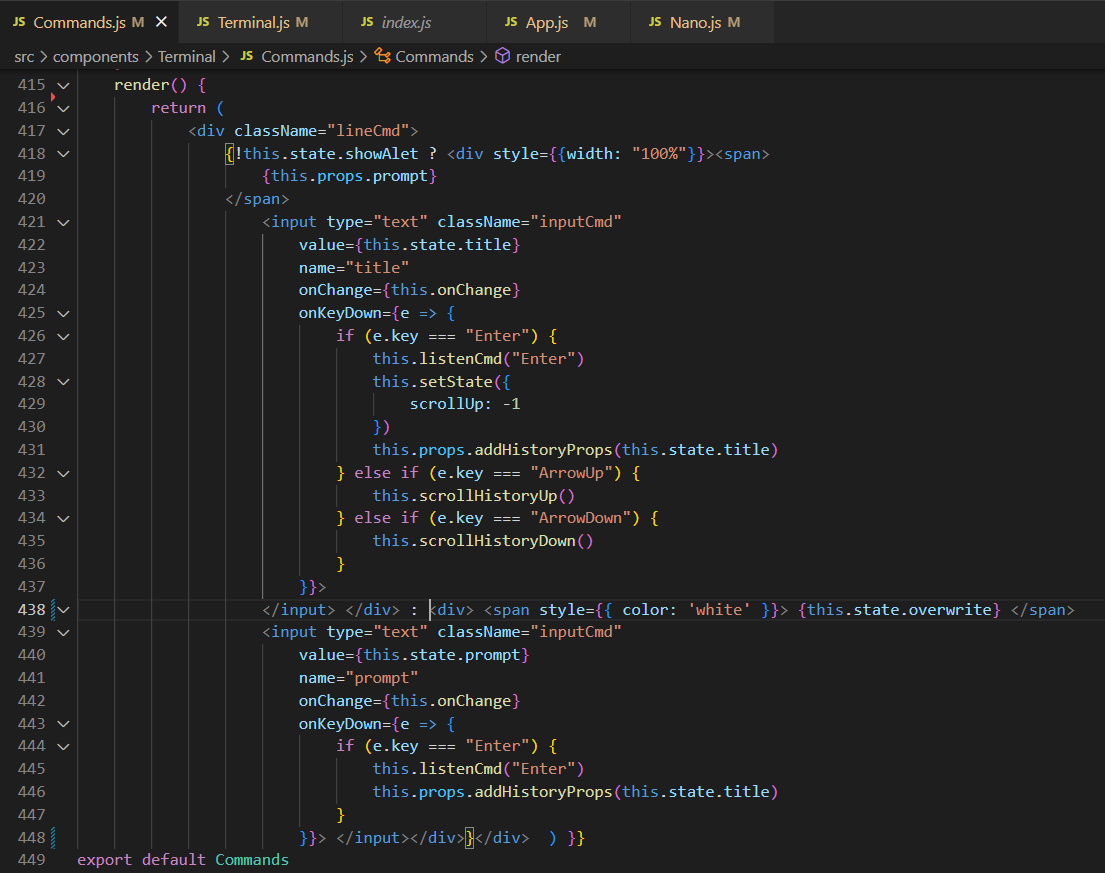
\includegraphics[width=370px]{code/command.png}
\begin{lstlisting}[escapeinside=``,caption={Renderowanie w komponencie Commands}]
`\vspace{-0.5cm}`
\end{lstlisting}
\end{center}
\vspace{0.1cm}
\begin{center}
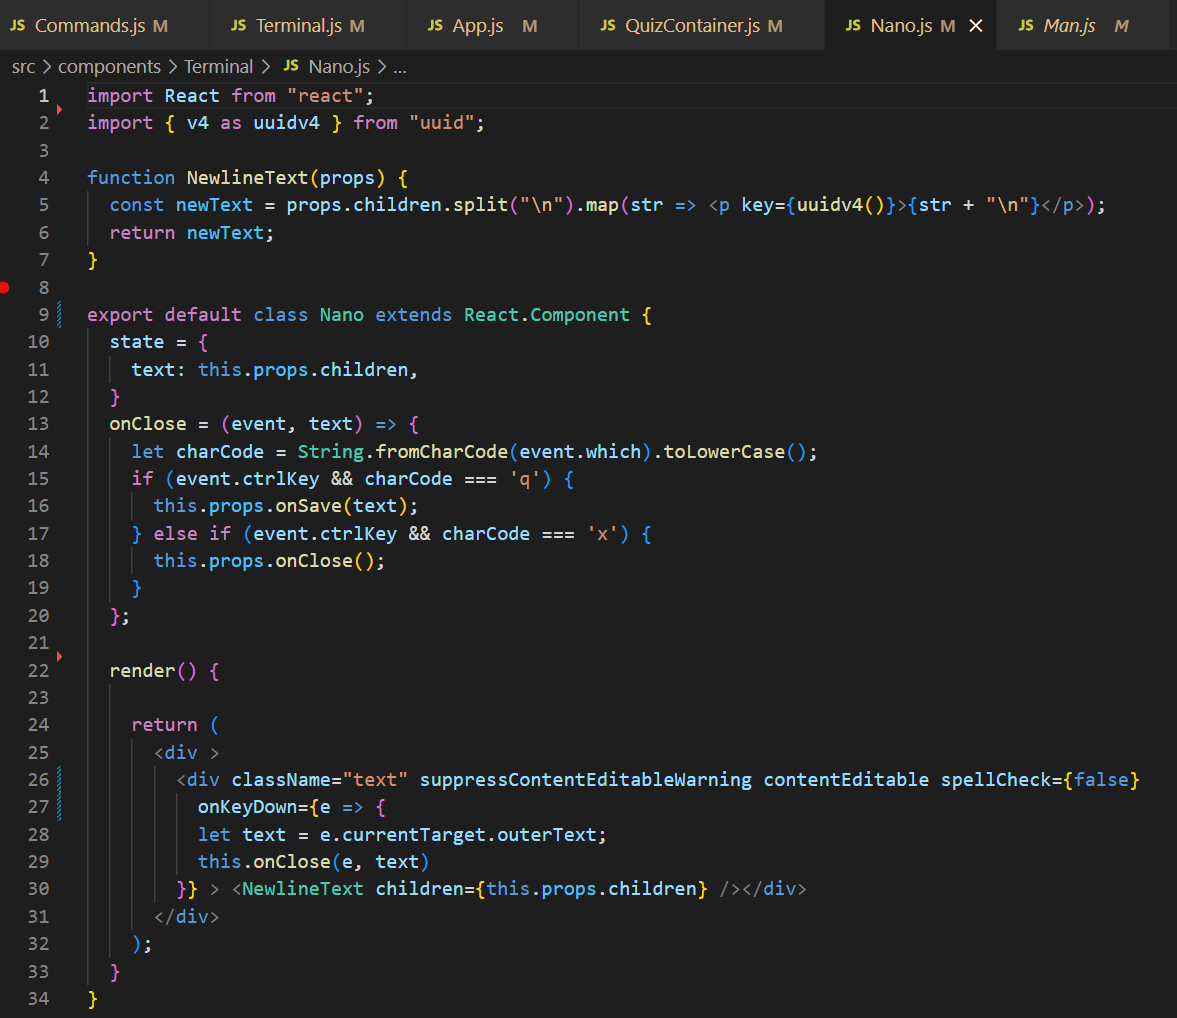
\includegraphics[width=350px]{code/nano.png} 
\begin{lstlisting}[escapeinside=``,caption={Komponent Nano użyty w projekci}]
`\vspace{-1cm}`
\end{lstlisting}
\end{center}
\begin{minipage}{1\linewidth}
Komponent Nano (Listing 3.3) służy do renderowania okna wyświetlającego edytor tekstowy nano. Ten komponent pozwala użytkowniku dodawać nowe dane lub modyfikować już istniejące w wybranym pliku. Okno edytora pojawia się po tym jak użytkownik wprowadzi polecenie "nano", jednocześnie jest sprawdzane czy dany plik już istnieje i czy są tam jakieś dane jeśli nie to jest tworzony nowy plik w którym zostaną zapisane dane wprowadzone przez użytkownika. Podczas renderowania w komponencie Nano sa tez nasłuchiwane zdarzenia klawiatury i po wybraniu odpowiedniego skróty jest wykonywana jakaś czynność np. Ctrl+q zapisuje wprowadzone dane w konkretnym pliku, a skrót Gtrl+x zamyka okno edytora i powraca do okna imitującego zachowanie terminala Linux.
\end{minipage}
\subsection{Routing wykorzystany w aplikacji}
\begin{minipage}{1\linewidth}
W aplikacji zostało wykorzystane narzędzie React Router(Listing 3.4) umożliwiające obsługę tras w aplikacji internetowej przy użyciu routingu dynamicznego. Routing dynamiczny wykorzystuje się podczas renderowania aplikacji. Switch i Route używane sa razem do mapowania docelowego adresu URL na komponent. Wraz z komponentem routera, router React zapewnia możliwość ustawienia i uzyskania dynamicznych informacji z adresu URL.
Na przykład do adresu URL może być dołączone id konkretnego elementu, który zostanie użyty do pobrania określonych obiektów. 
\end{minipage}
\vspace{0.3cm}
\begin{center}
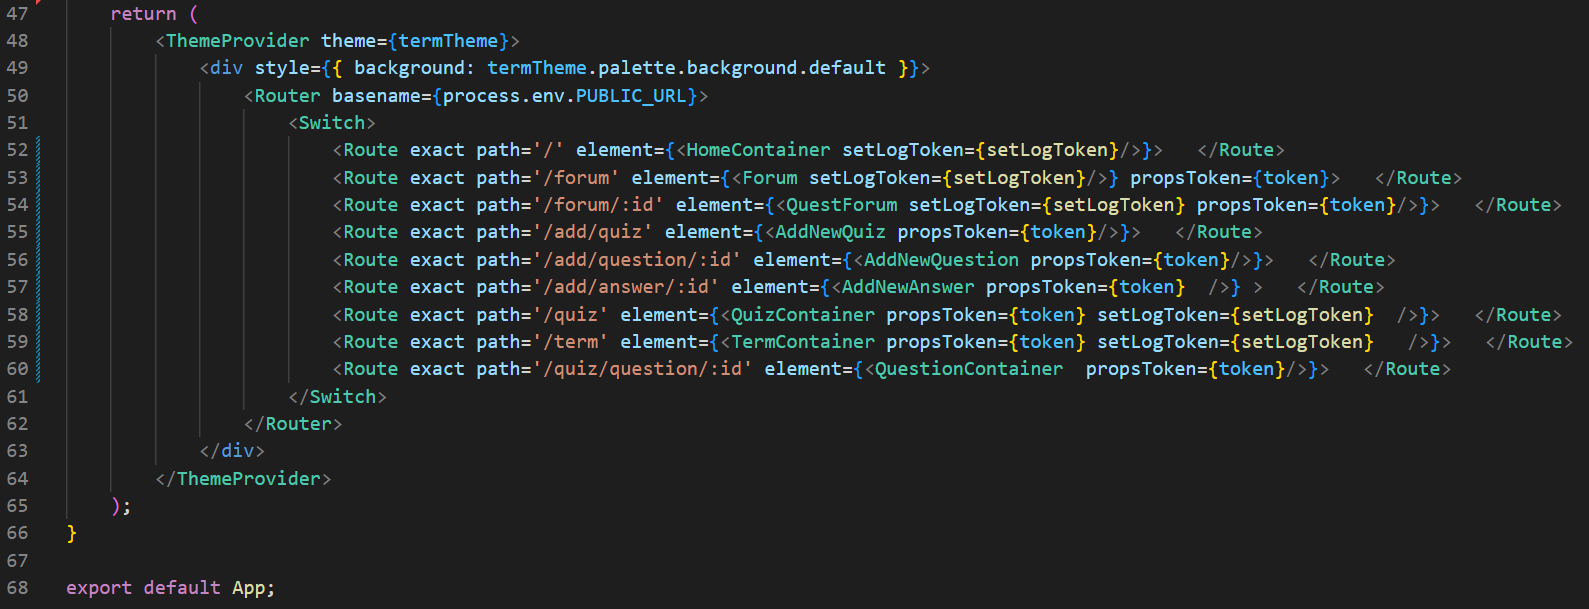
\includegraphics[width=350px]{code/routers.png} 
\begin{lstlisting}[escapeinside=``,caption={Routing użyty w projekcie}]
`\vspace{-1.2cm}`
\end{lstlisting}
\end{center}
\section{Interfejs Użytkownika}
\subsection{Widok strony głównej}
\begin{minipage}{\linewidth}
\begin{center}
  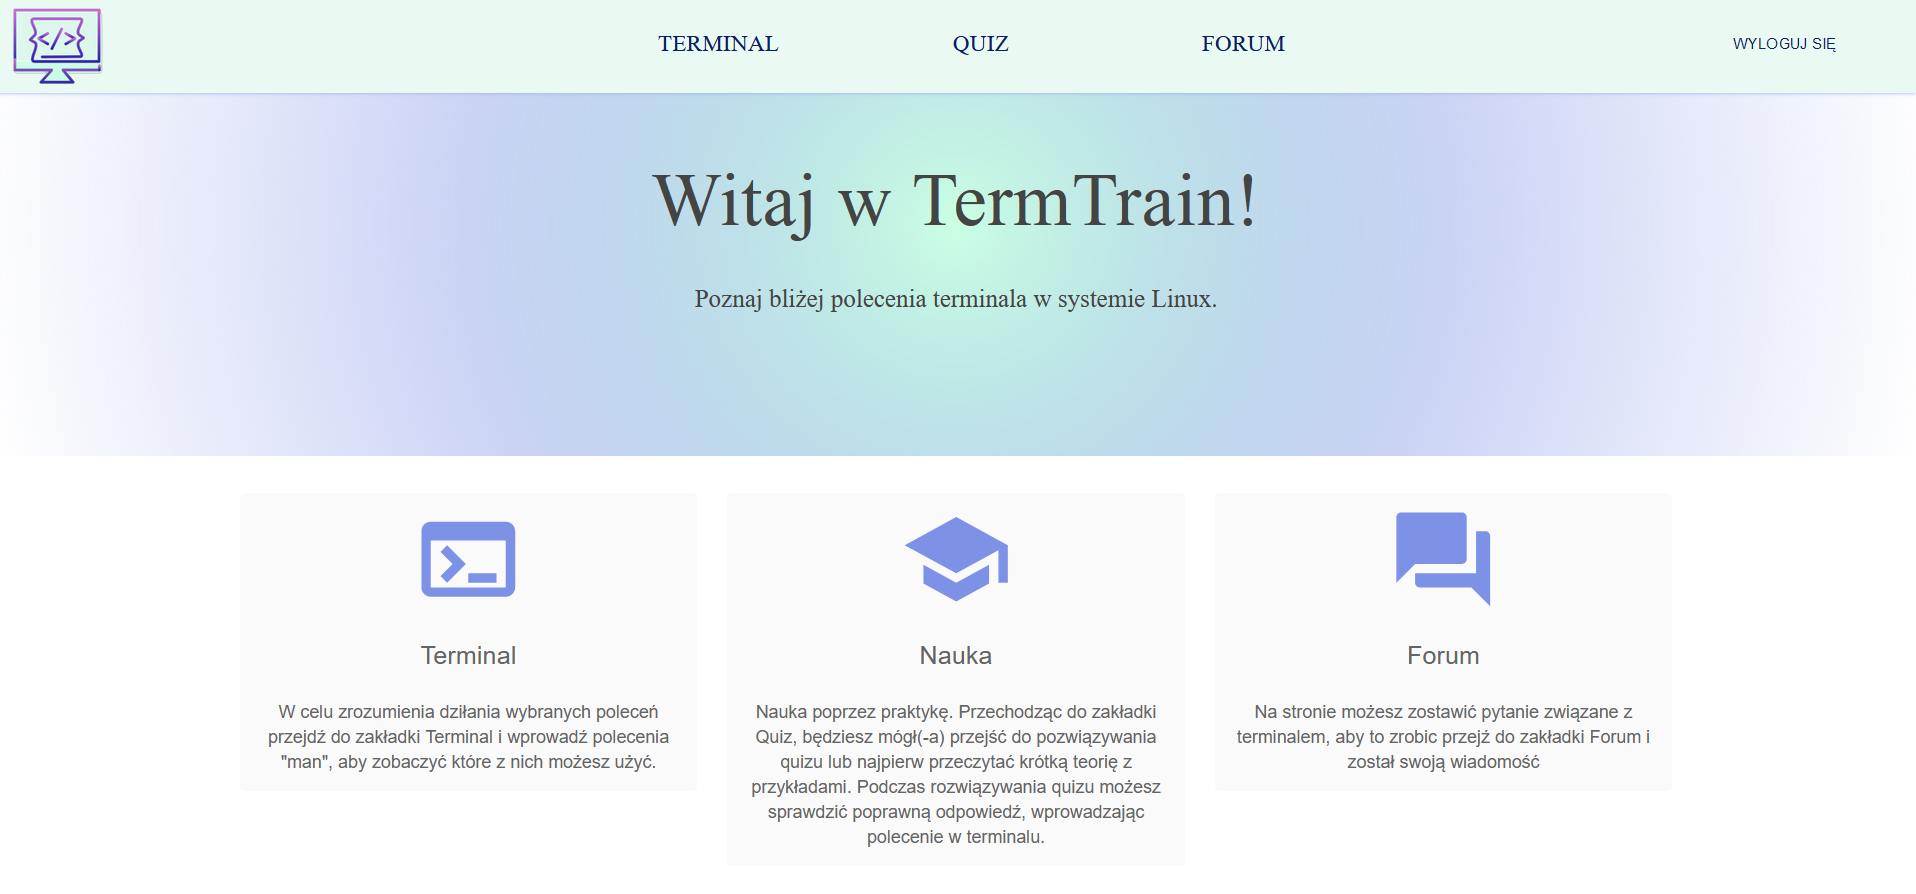
\includegraphics[width=400px]{project/main_page.png}
  \captionof{figure}{ \textit{Widok ekranu głównego aplikacji}} 
\end{center}
\end{minipage}
\begin{minipage}{1\linewidth}
\vspace{0.3cm}
Na stronie głównej aplikacji jest widoczny jej krótki opis oraz
pasek menu, na którym znajdują się zakładki otwierające podstawowe strony aplikacji.
Zakładka Terminal otwiera stronę z oknem  imitującym zachowanie terminala Linux, zakładka Quiz przenosi
użytkownika do widoku listy quizów, zakładka Forum przenosi użytkownika do strony
wyświetlającej listę pytań oraz przycisk wylogowania.
\end{minipage}
\begin{multicols}{2}
[
\subsection{Widok logowania oraz rejestracji}
Każdy użytkownik chcący korzystać z aplikacji TermTrrain powinien mieć utworzone konto, oraz być zalogowanym.
]
\begin{minipage}{\linewidth}
  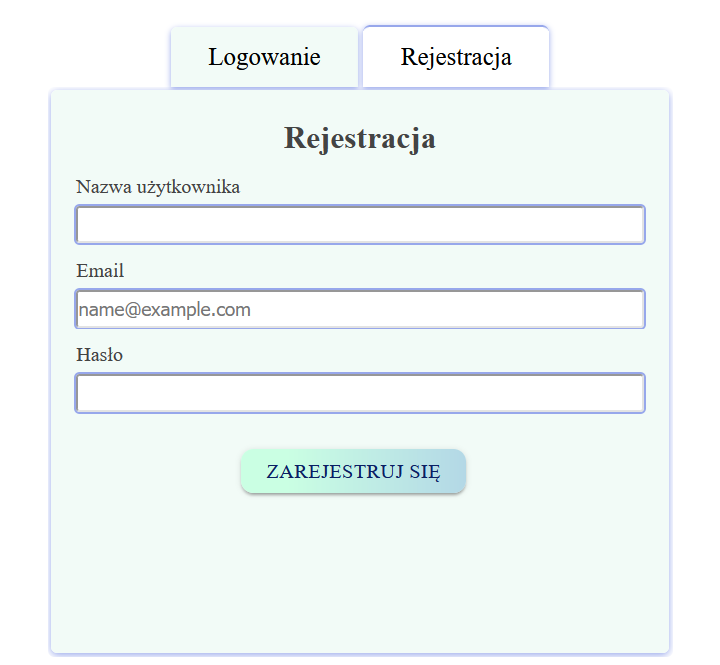
\includegraphics[width=200px]{project/rejestracja.png}
  \captionof{figure}{ \textit{Widok ekranu rejestracji}} 
\end{minipage}

\begin{minipage}{\linewidth}
  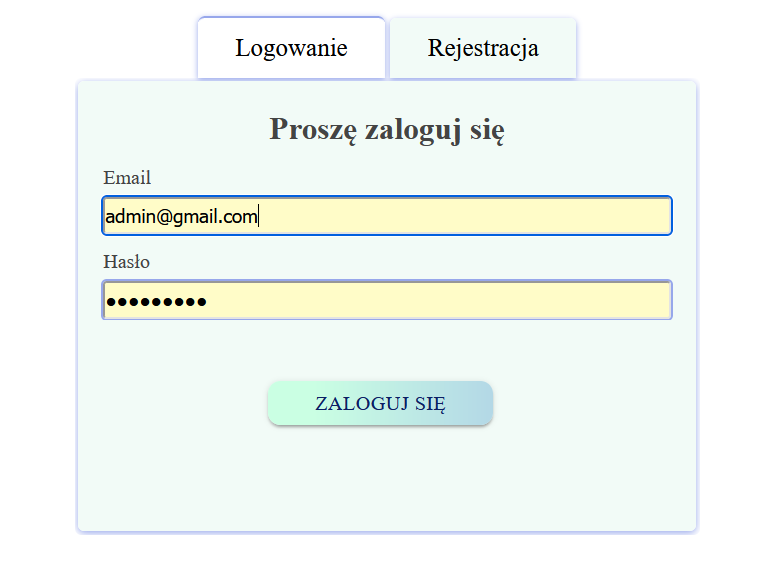
\includegraphics[width=210px]{project/logowanie.png}
  \captionof{figure}{ \textit{Widok ekranu logowania}} 
\end{minipage}
\end{multicols}
\subsection{Widok okna terminala}
\begin{minipage}{1\linewidth}
Po wybraniu zakładki Terminal w pasku głównym menu, zostanie wyświetlone okno imitujące zachowanie terminala Linux.
Z prawej strony terminala znajduje się pasek menu, podobny do tego na stronie głównej, z wyjątkiem jednej zakładki służącej do przejścia na stronę główną. \\
\end{minipage}

\begin{minipage}{\linewidth}
\begin{center}
  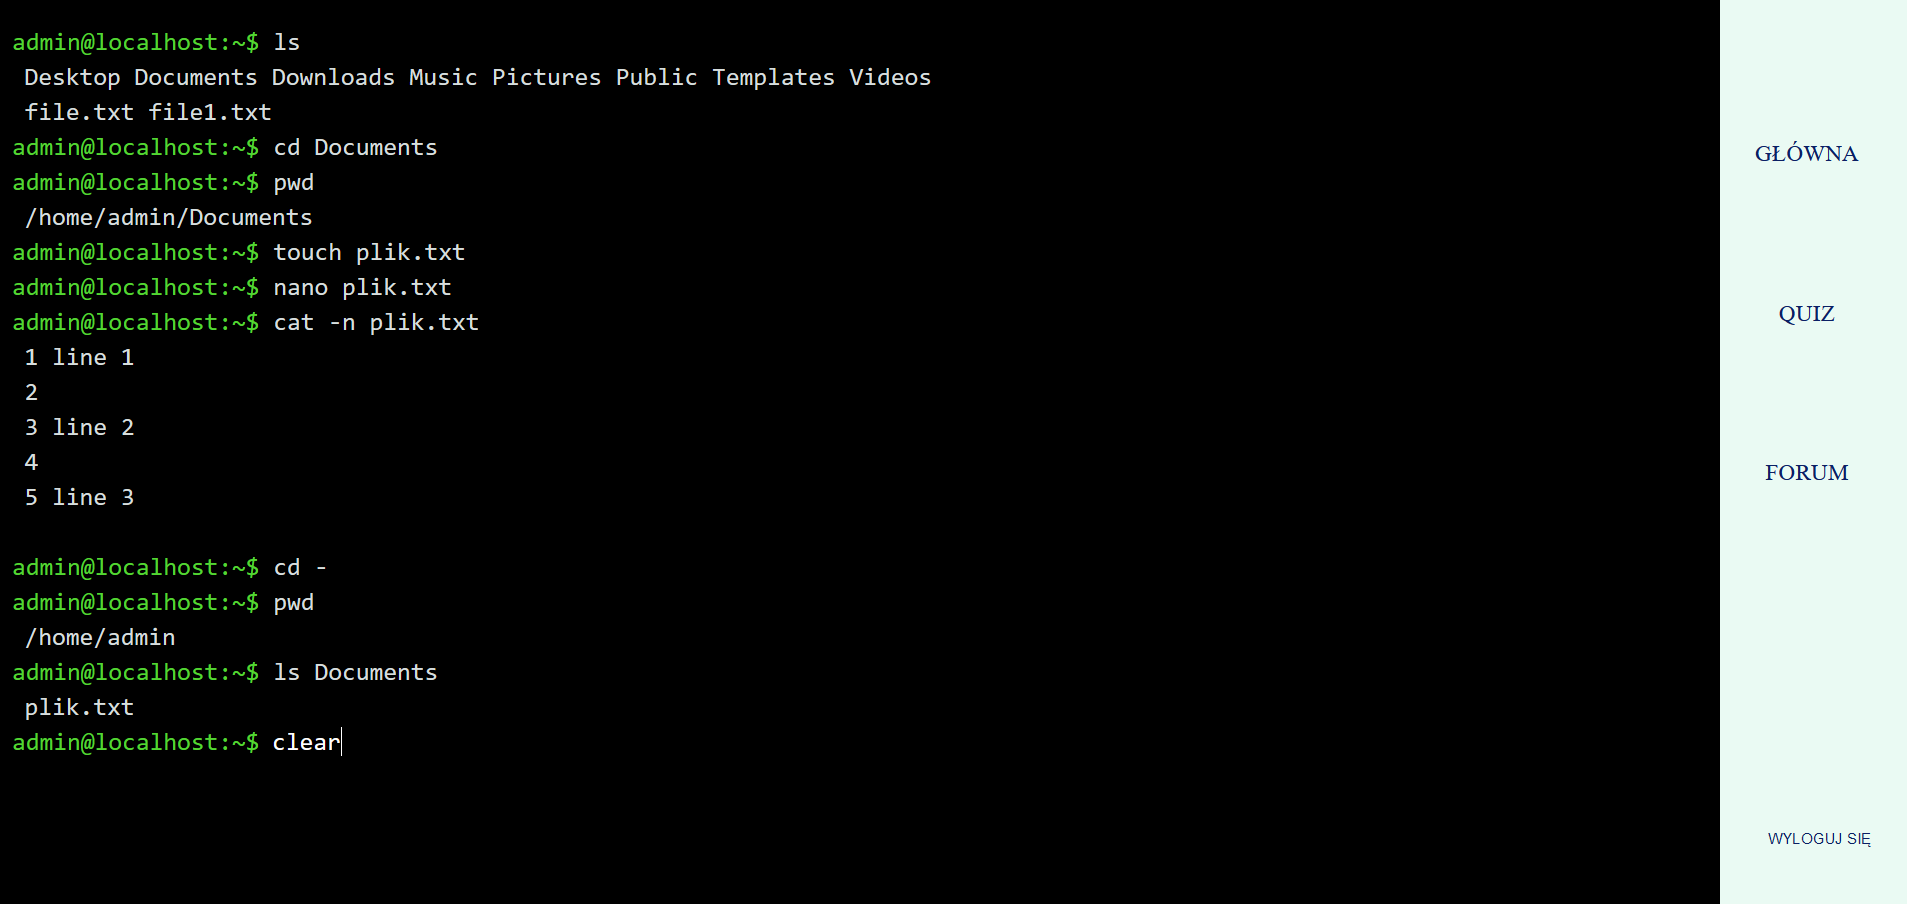
\includegraphics[width=400px]{project/term1.png}
  \captionof{figure}{ \textit{Widok okna terminala z przykładowym użyciem poleceń}} 
\end{center}
\end{minipage}
\begin{minipage}{1\linewidth}
\vspace{0.3cm}
 Terminal skład się z wiersza poleceń, który zawiera przydatne informacje dla użytkownika, takie jak nazwa aktualnie zalogowanego użytkownika, symbol "@" który jest separatorem pomiędzy nazwą użytkownika a nazwą hosta, symbol "$\sim$" reprezentuje katalog domowy aktualnie zalogowanego użytkownika, symbol \$ oznacza, że użytkownik jest zalogowany 
  \end{minipage}
  \begin{minipage}{1\linewidth}
 jako zwykły użytkownik, jeżeli użytkownik jest zalogowany jako "root" ten 
 symbol zmieni się na symbol "\#".\\  \\
 Jeśli użytkownik wprowadzi jedno z dozwolonych poleceń, taki jak: ls, cd, pwd, rm, rmdir, mkdir, touch, cat, echo, nano, man, mv, cp to w oknie terminala wyświetlą się odpowiednie dane wyjściowe, symulując tym samym działania konkretnego polecenia, np. wypisując listę plików i katalogów, nazwę aktualnego katalogu lub zawartość pliku itp. \\ 
 \end{minipage}
\begin{minipage}{\linewidth}
\begin{center}
  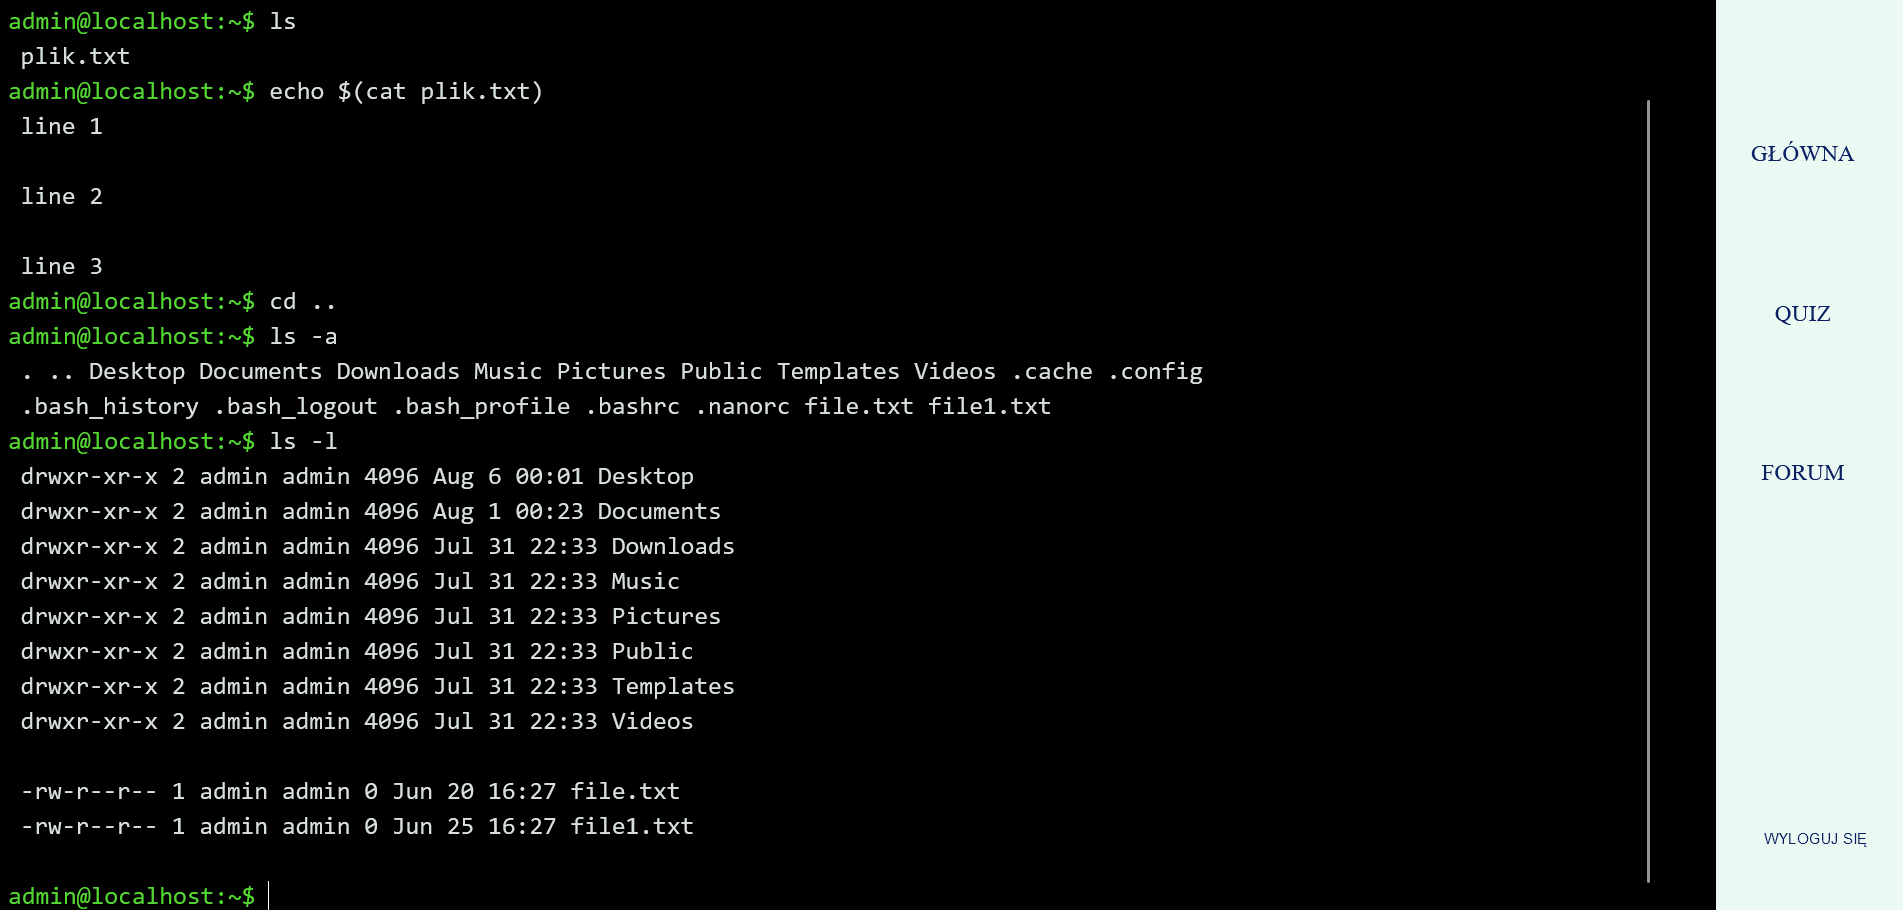
\includegraphics[width=400px]{project/term2.png}
  \captionof{figure}{ \textit{Widok okna terminala z przykładowym użyciem poleceń}} 
\end{center}
\end{minipage}
\begin{minipage}{1\linewidth}
\vspace{0.3cm}
Użytkownik może wykorzystać komendę "man nazwa\_polecenia", aby dowiedzieć się więcej o danym poleceniu. Polecenie man służy otwierania interfejsu stron podręcznika ekranowego zawierającą podstawowe informacje o konkretnym poleceni.
Żeby dowiedzieć się jakie polecenia można wykorzystywać w imitacji terminala Linux, wystarczy wpisać w wierszu poleceń komendę "mam", której działaniem będzie wyświetlenie strony zawierającej informację o tych poleceniach. Jeśli użytkownik będzie chciał zamknąć interfejs strony podręcznika ekranowego oraz powrócić do imitacji wiersza poleceń wystarczy, że naciśnie na klawisz "q".\\ \\
\end{minipage}
\begin{minipage}{\linewidth}
\begin{center}
  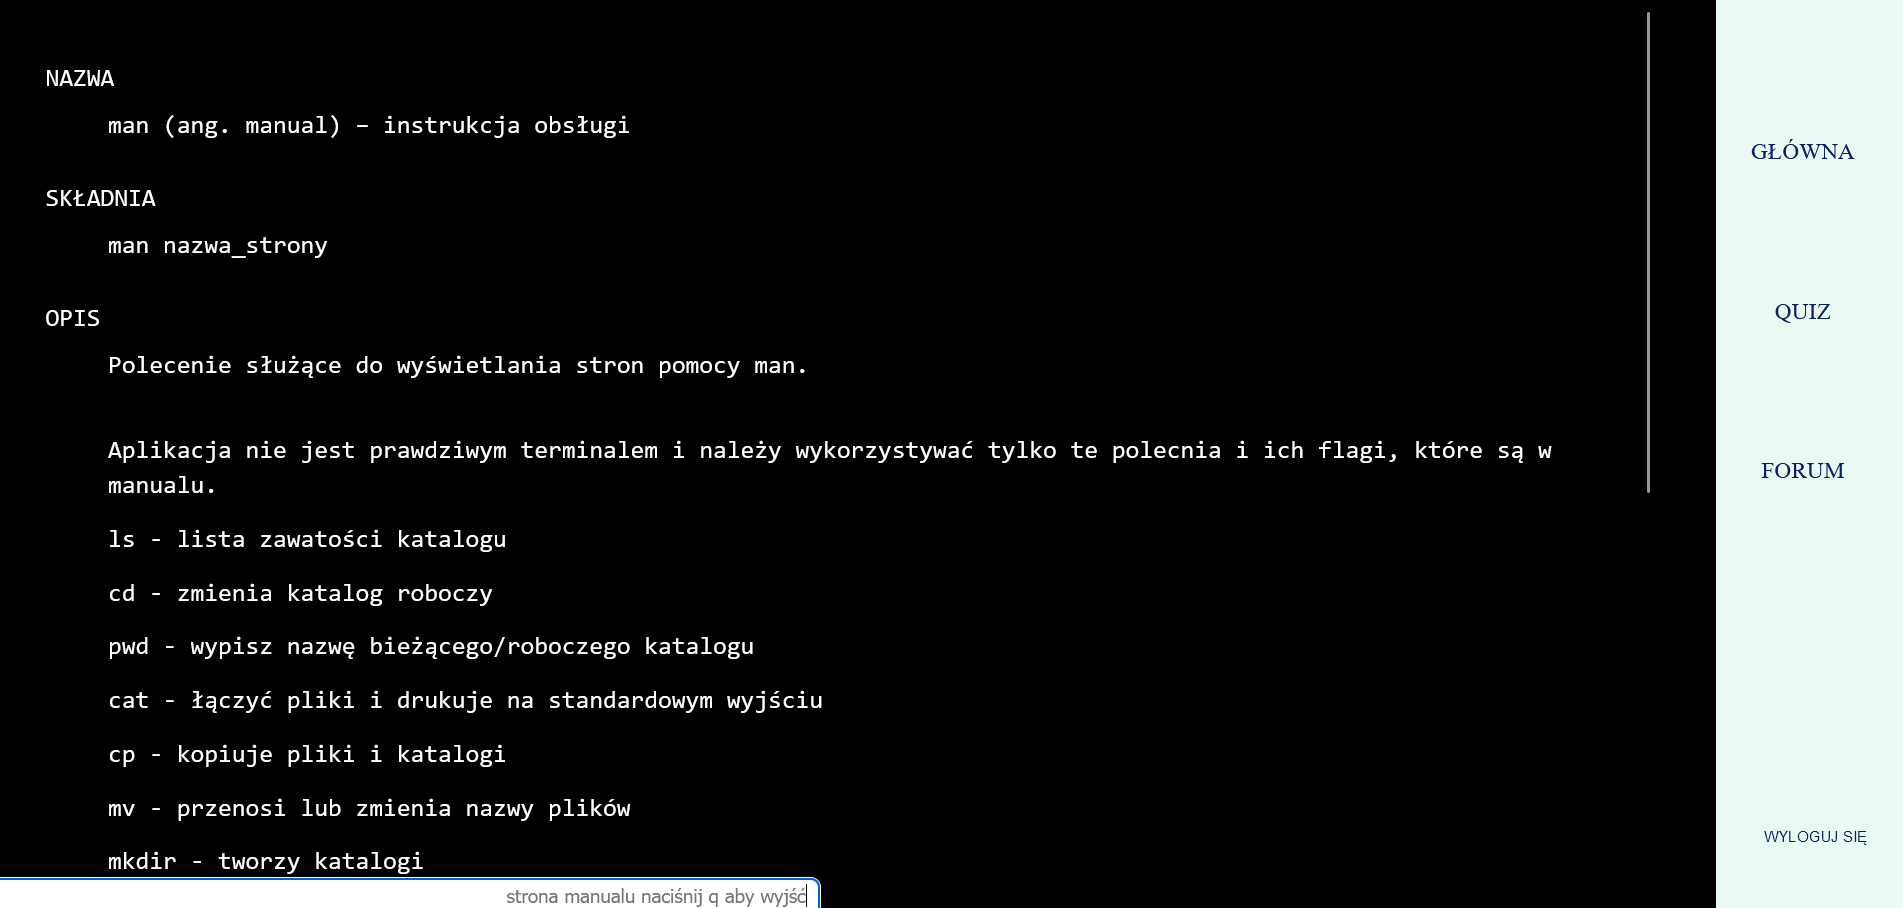
\includegraphics[width=400px]{project/man.png}
  \captionof{figure}{ \textit{Widok okna terminala z przykładowym użyciem polecenia man}} 
\end{center}
\end{minipage}
\subsection{Widok ekranu wyświetlającego listę quizów}
\begin{minipage}{1\linewidth}
Po wybraniu zakładki Quiz  w pasku głównym menu, użytkownikowi zostaje wyświetlona lista quizów.
Widoczne są nazwy quizów oraz przyciski jeden, z których umożliwia przejście do rozwiązania quizu, a drugi otwiera okno wyświetlające informację o poleceniach znajdujących się w konkretnym quizie.\\  \\
\end{minipage}
\begin{minipage}{\linewidth}
\begin{center}
  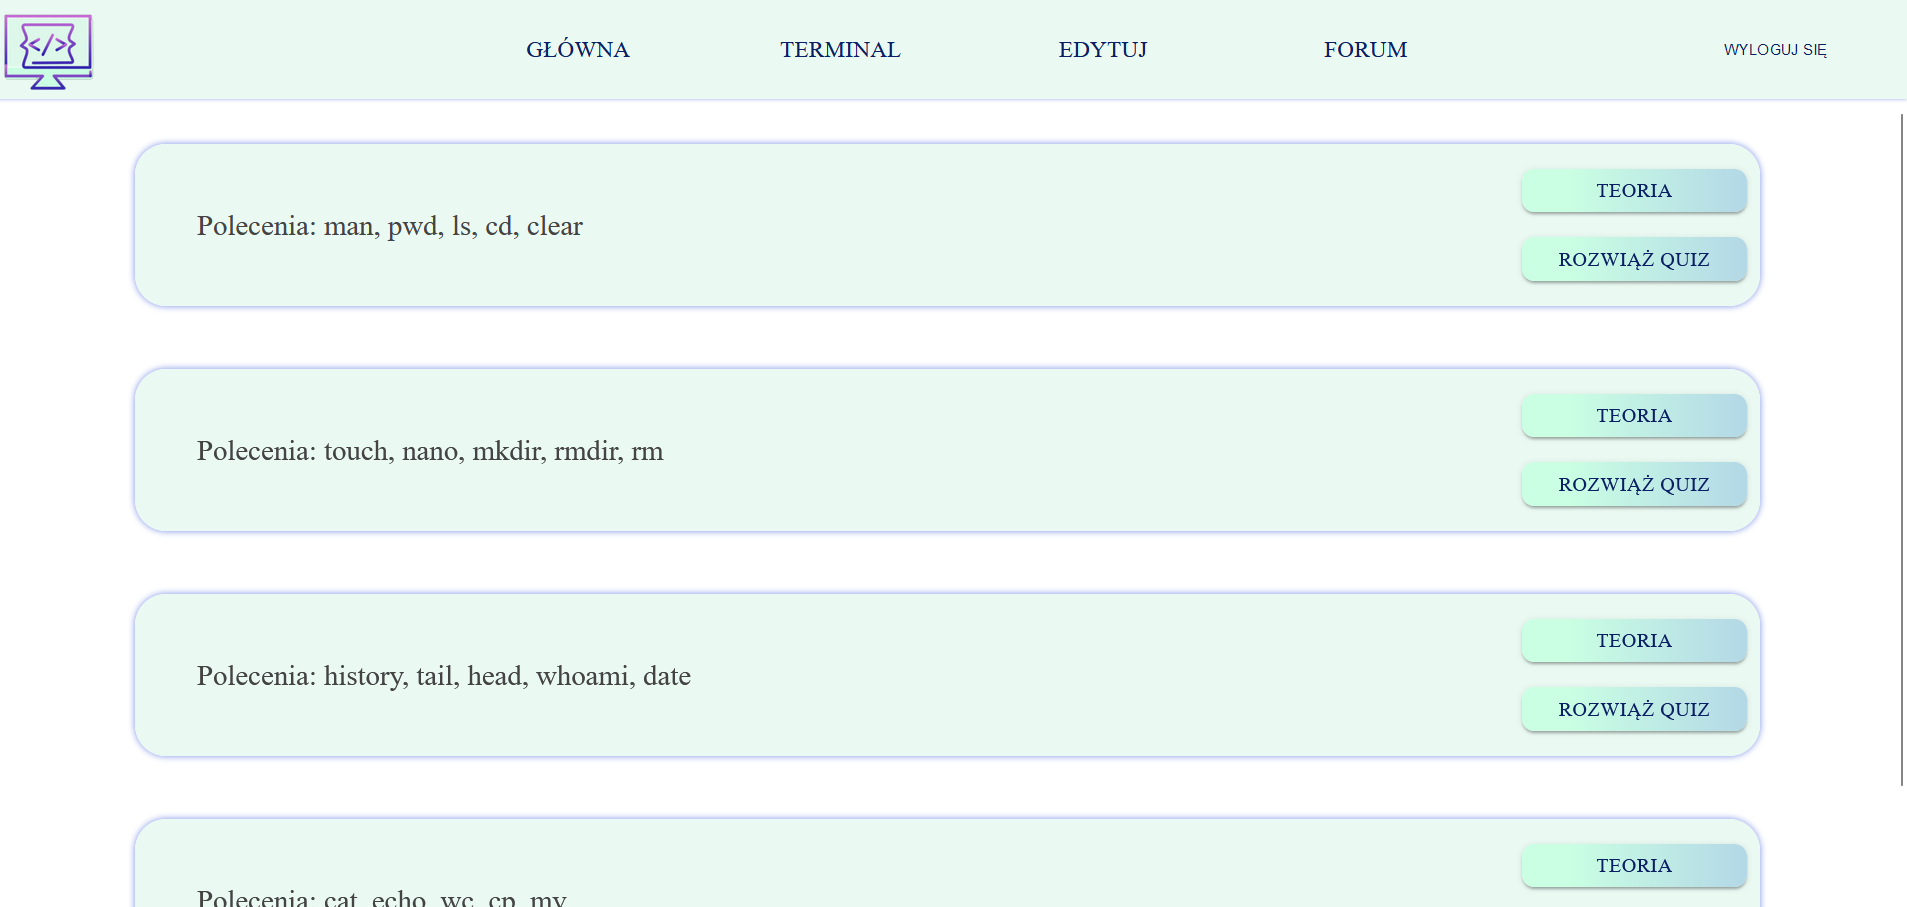
\includegraphics[width=300px]{project/list_quiz.png}
  \captionof{figure}{ \textit{Widok ekranu wyświetlającego listę quizów}} 
\end{center}
\end{minipage}
\begin{minipage}{1\linewidth}
\vspace{0.3cm}
 Po rozwiązaniu quizu wyniki uzyskane przez użytkownika wyświetlane są po prawej stronie przycisków, po ponownym przejściu quizu wyniki są aktualizowane. \\ 
\end{minipage}
\begin{minipage}{\linewidth}
\begin{center}
  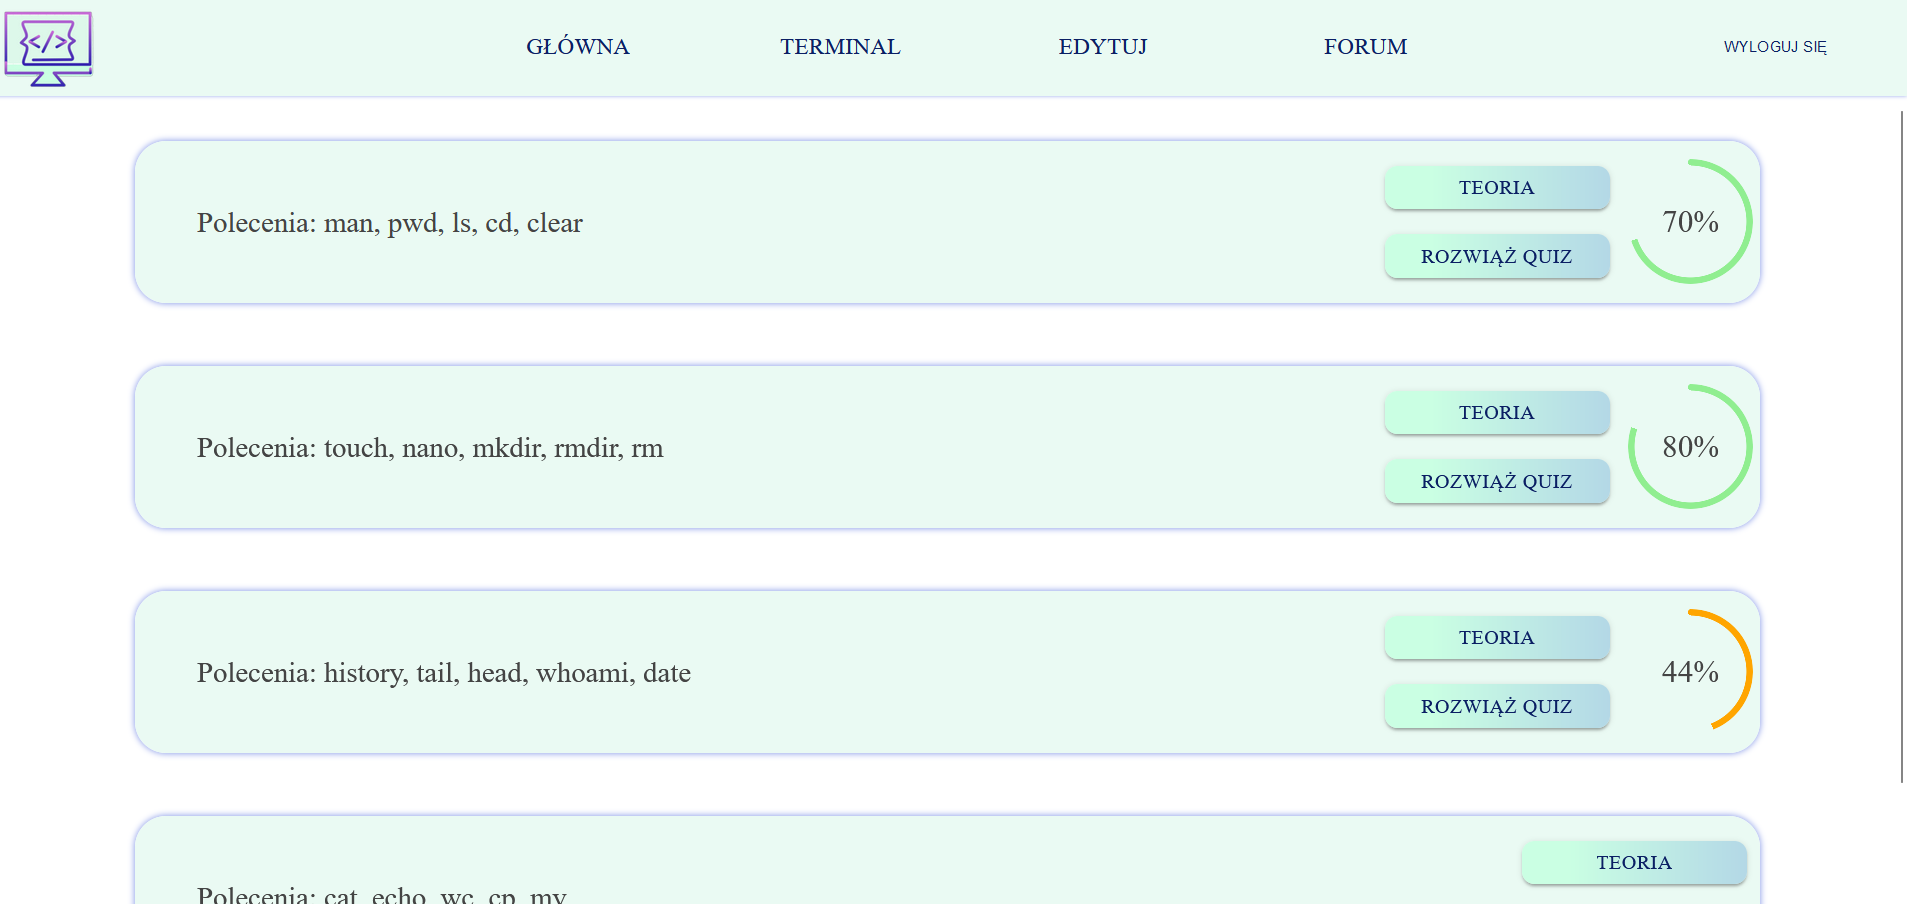
\includegraphics[width=300px]{project/list_quiz2.png}
  \captionof{figure}{ \textit{Widok ekranu wyświetlającego listę  quizów oraz wyniki}} 
\end{center}
\end{minipage}
\begin{minipage}{1\linewidth}
\vspace{0.3cm}
Przed rozwiązywanie quizu użytkownik może opcjonalnie przeczytać krótki opis oraz przykłady poleceń, które są zawarte w konkretnym quizie.\\
\end{minipage}
\begin{minipage}{\linewidth}
\begin{center}
  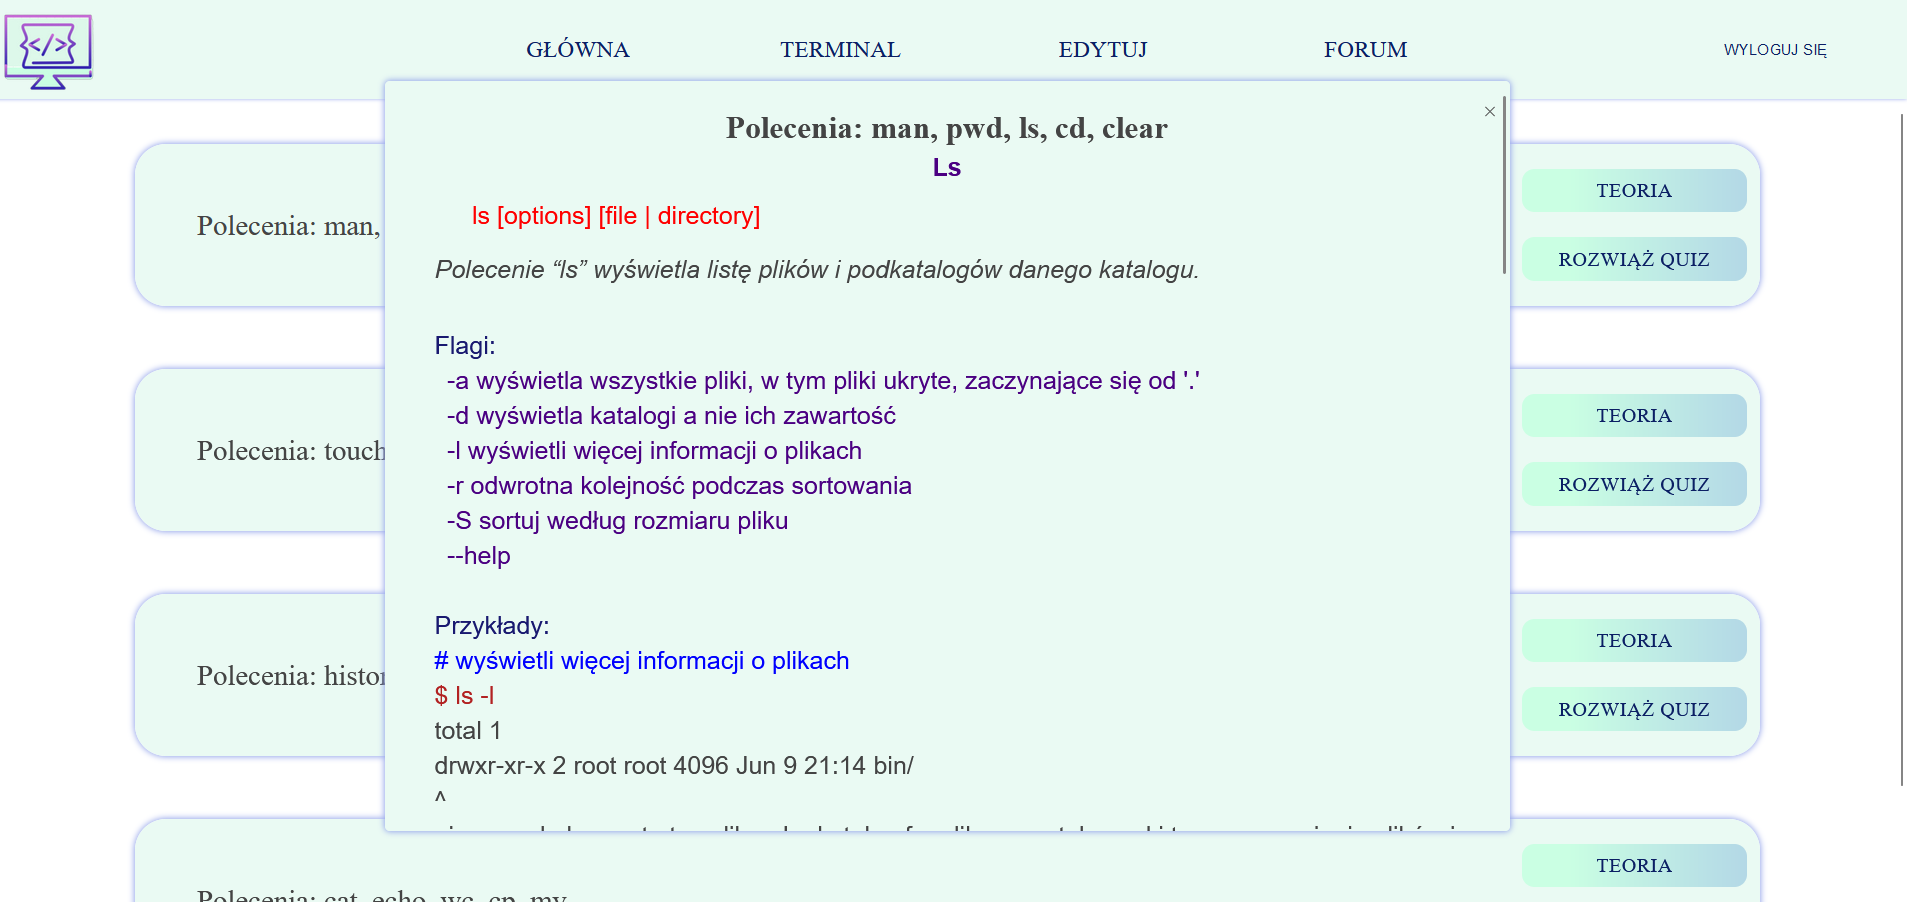
\includegraphics[width=300px]{project/teoria.png}
  \captionof{figure}{ \textit{Widok okna wyświetlającego informacje o poleceniach zawartych w quizie}} 
\end{center}
\end{minipage}
\subsection{Widok konkretnego quizu}
\begin{minipage}{1\linewidth}
W widoku listy quizów użytkownik może wybrać opcje rozwiązanie quizu, po czym zostanie przeniesiony do widoku quizu. Podczas rozwiązywania quizu użytkownik może wybierać jedną z możliwych odpowiedzi i przechodzić do następnego pytania. Poza tym użytkownik może sprawdzać poprawną odpowiedź, sprawdzając każde polecenie w imitacji wiersza poleceń znajdującego się po lewej stronie quizu. \\
\end{minipage}
\begin{minipage}{\linewidth}
\begin{center}
  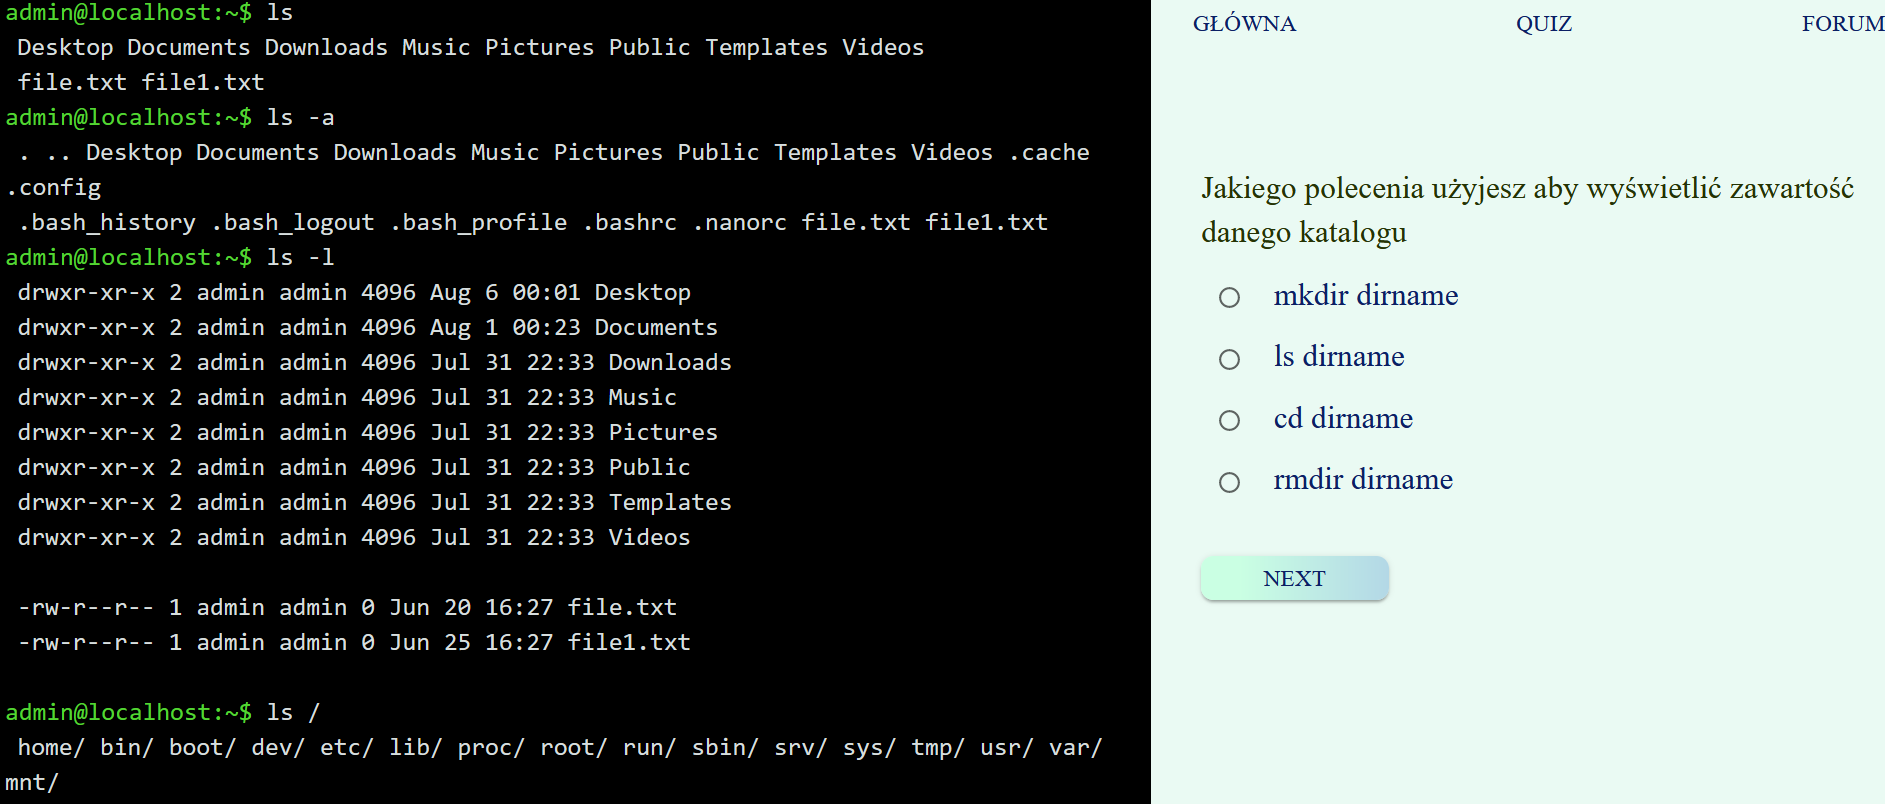
\includegraphics[width=400px]{project/quiz1.png}
  \captionof{figure}{ \textit{Widok  konkretnego quizu oraz terminala }} 
\end{center}
\end{minipage}
\begin{minipage}{1\linewidth}
\vspace{0.3cm}
 Po zakończeniu każdego quizu jest wyświetlany wynik końcowy, który później jest widoczny w widoku listy quizów. \\
 \end{minipage}
\begin{minipage}{\linewidth}
\begin{center}
  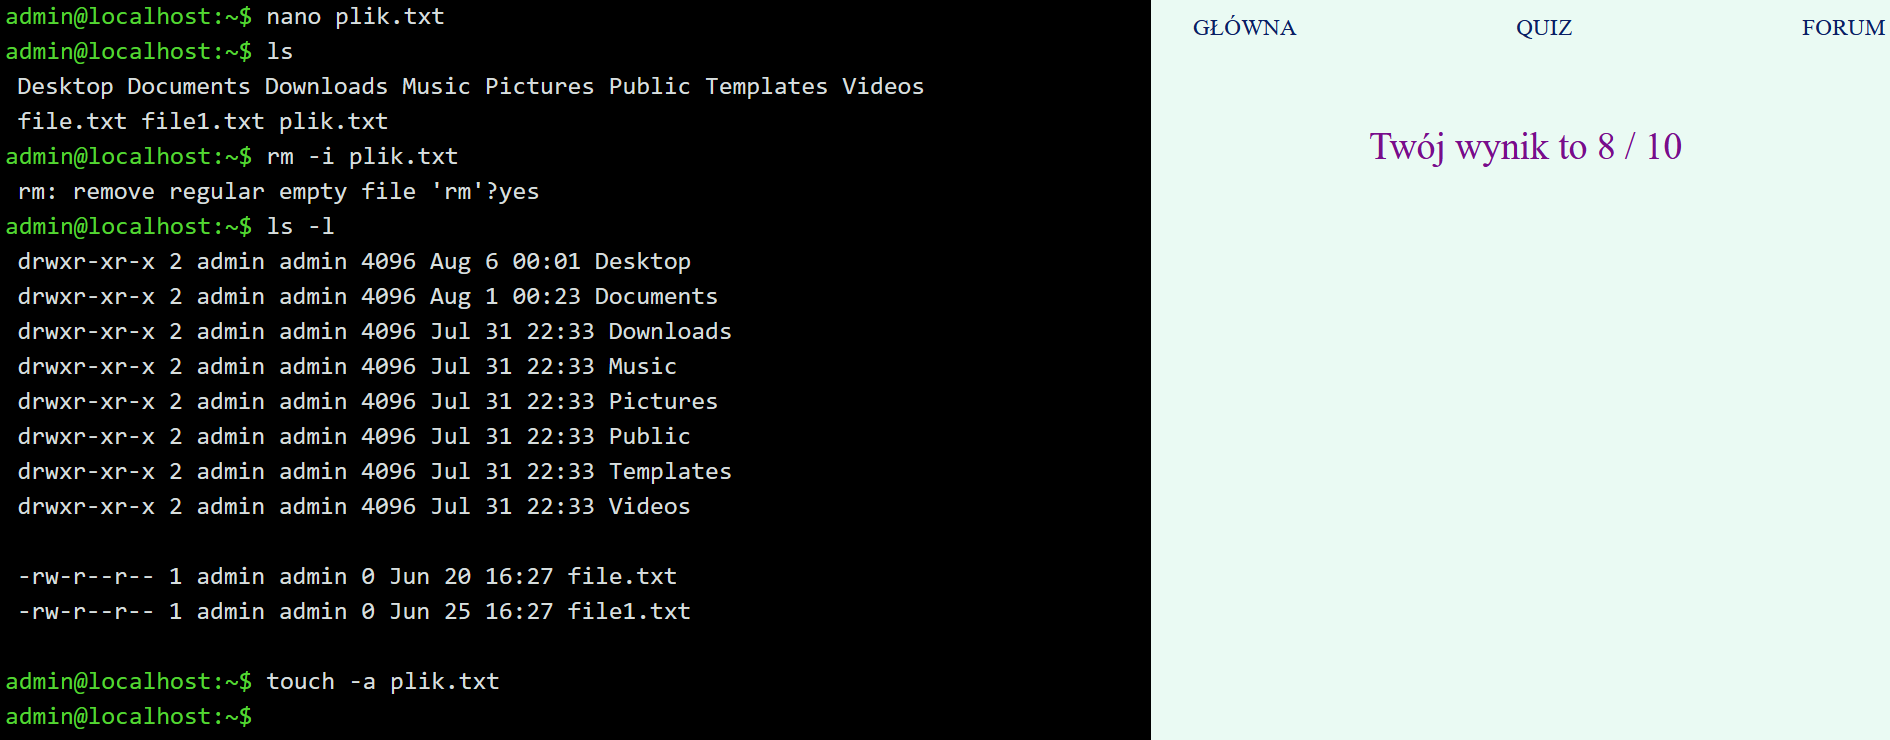
\includegraphics[width=400px]{project/quiz2.png}
  \captionof{figure}{ \textit{Wyniku wyświetlany po przejściu konkretnego quizu}} 
\end{center}
\end{minipage}
\begin{minipage}{1\linewidth}
\vspace{0.3cm}
Jeżeli użytkownik jest zalogowany jako administrator, to na pasku menu zakładki quiz jest widoczna zakładka "edytuj" która przenosi użytkownika do strony służącej do dodawania oraz usuwania quizów.\\ 
\end{minipage}
\begin{minipage}{\linewidth}
\begin{center}
  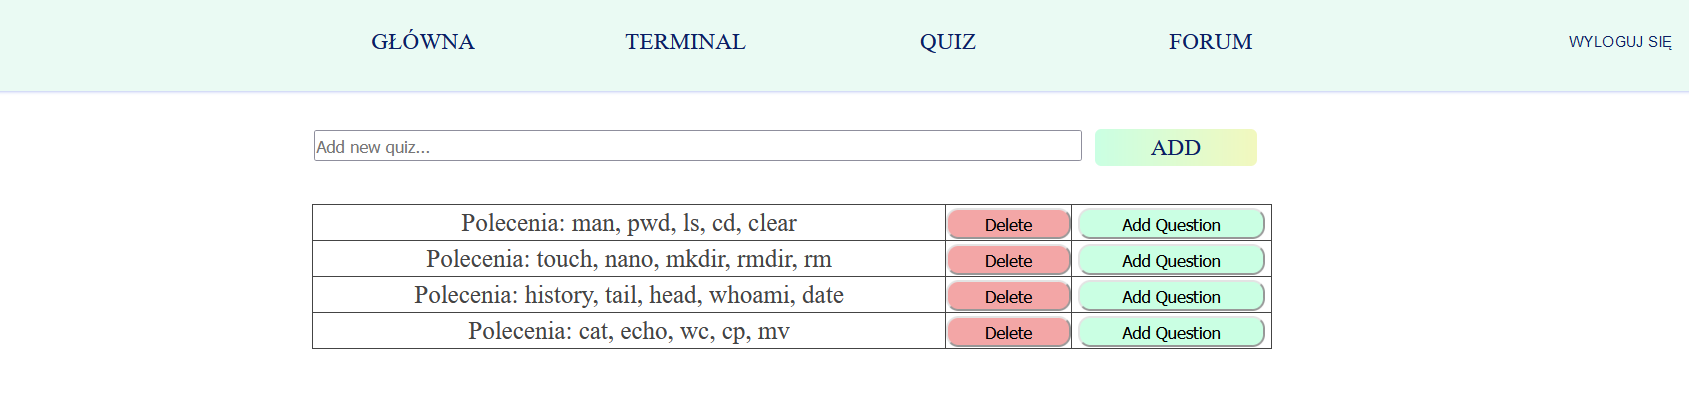
\includegraphics[width=400px]{project/add_quiz.png}
  \captionof{figure}{ \textit{Widok okna przeznaczonego do dodawania oraz usuwania quizów}} 
\end{center}
\end{minipage}
\subsection{Widok listy pytań na forum}
\begin{minipage}{1\linewidth}
Po wybraniu zakładki Forum w pasku głównym menu, użytkownikowi zostaje wyświetlona lista pytań na forum. W prawym górnym rogu strony znajduje się przycisk w wyglądzie plusa, który służy do dodania nowych pytań na forum. Po kliknięciu tego przycisku przed użytkownikiem zostanie wyświetlone okno z formularzem, który składa się z dwóch pól, w pierwszym wpisuje się pytanie, a w drugim szczegółowy opis tego pytania. \\ 
\end{minipage}
\begin{minipage}{\linewidth}
\begin{center}
  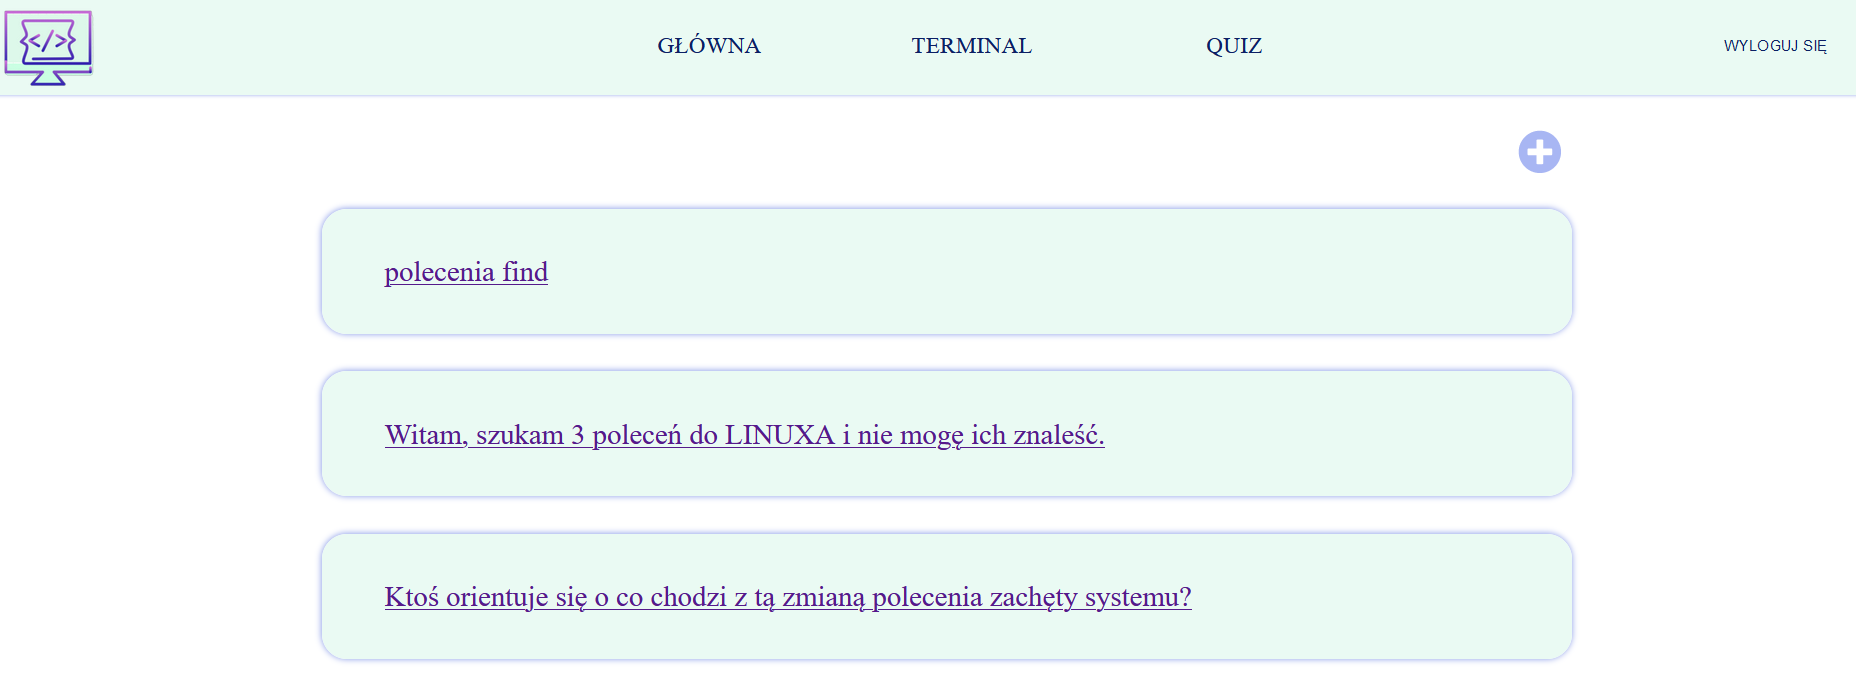
\includegraphics[width=350px]{project/forum.png}
  \captionof{figure}{ \textit{Widok listy pytań na forum}} 
\end{center}
\end{minipage}
\begin{minipage}{1\linewidth}
\vspace{0.3cm}
Po wyborze konkretnego pytania na forum użytkownik zostaje przeniesiony do widoku opisu konkretnego pytania. Znając odpowiedź na dane pytanie użytkownik może zostawić swój komentarz, pod konkretnym pytaniem lub też przejrzeć komentarzy innych użytkowników i polubić te, które na jego myśl są najlepszą odpowiedzią.\\
\end{minipage}
\begin{minipage}{\linewidth}
\begin{center}
  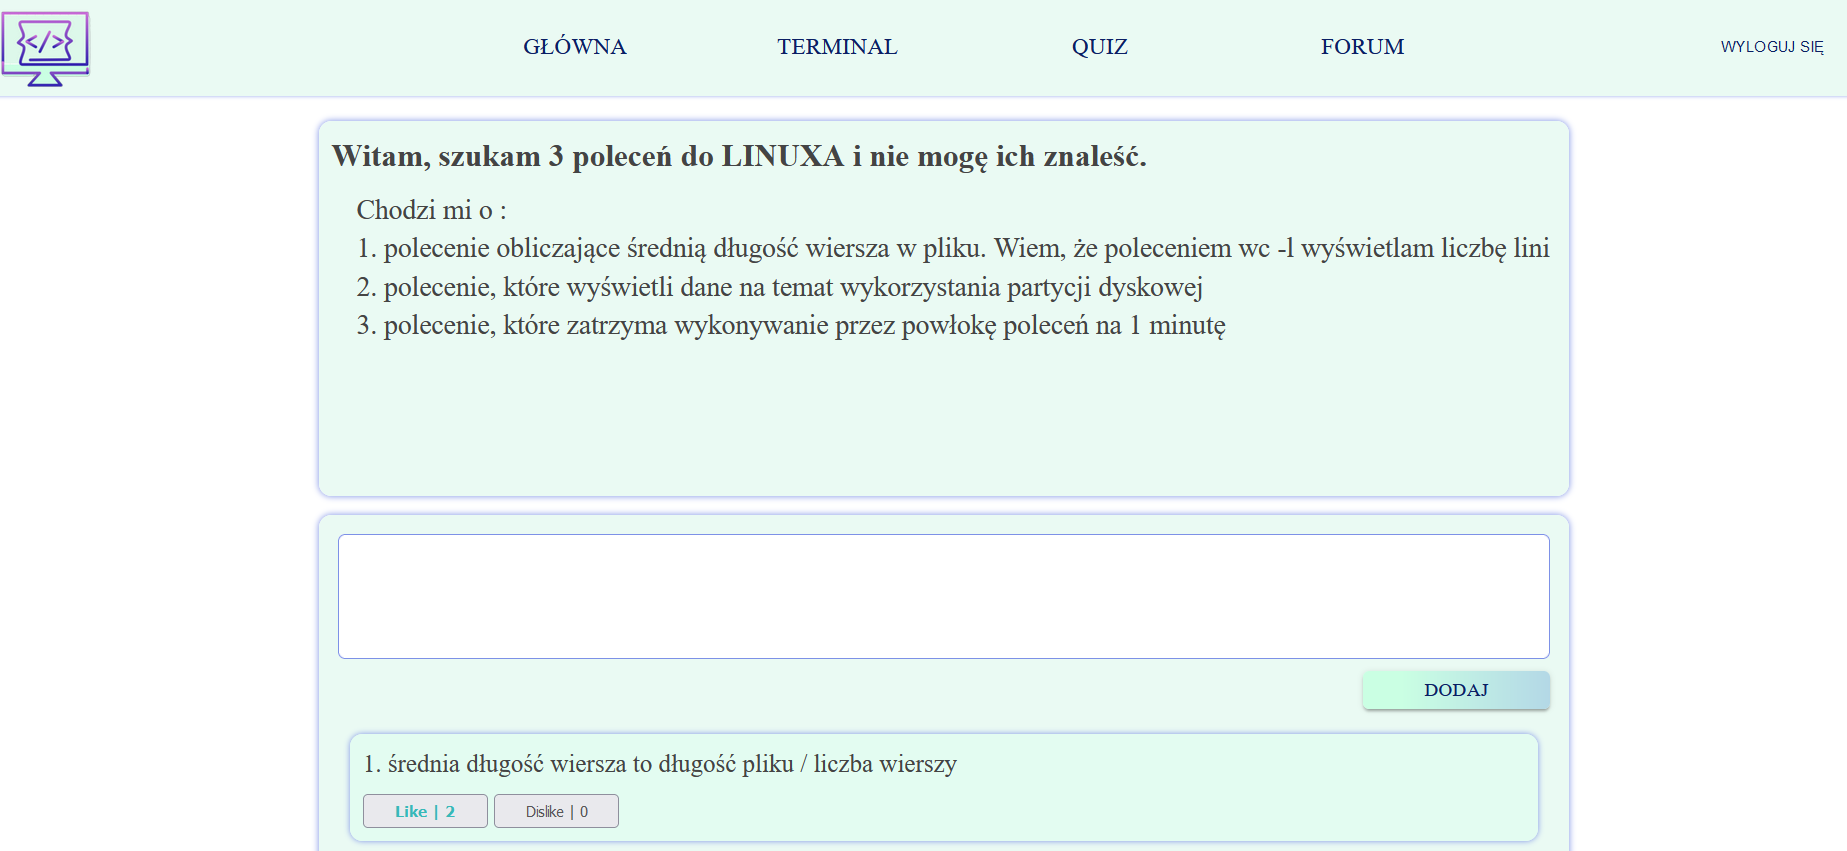
\includegraphics[width=350px]{project/quest_comment.png}
  \captionof{figure}{ \textit{Widok okna z opisem konkretnego pytania}} 
\end{center}
\end{minipage}
\chapter*{Podsumowanie}
\addcontentsline{toc}{chapter}{Podsumowanie}
\begin{minipage}{1\linewidth}
Cel pracy obejmował wykonanie projektu oraz implementacji aplikacji imitującej zachowanie konsoli Linux, która uprościłaby zwykłym użytkownikom naukę podstaw terminala. Projekt zakładał uruchamianie aplikacji w dowolnej przeglądarce, umożliwiając tym samym naukę przez praktykę bez konieczności instalowania systemu operacyjnego Linux lub jego uruchamianie na wirtualnej maszynie. \\ \\
Na początku przedstawiono krótką historie Linuxa i opisana została struktura systemu operacyjnego. Następnie zostały omówione narzędzia które zostały wykorzystane podczas pisania aplikacji. Oraz przedstawiono wstępne założenia aplikacji. \\ \\
W dalszej części zostały omówione poszczególne przypadki użycia oraz tabele baz danych. Następnie zostały omówione wybrane komponenty części frontendowej aplikacji. Na koniec zostały opisane poszczególne widoki interfejsu użytkownika aplikacji. \\ \\
Podsumowując, cel pracy został osiągnięty. Stworzona aplikacji pomyślnie działa oraz została zaprezentowana w niniejszy pracy. Działa prawidłowo, mimo to w przyszłości planuję ją udoskonalać i rozbudowywać. 
\end{minipage}

\addcontentsline{toc}{chapter}{Bibliografia}
\begin{thebibliography}{9}
\setlength\itemsep{0.3cm}
\bibitem{textbook}
\url{https://opensource.com/resources/linux } - odwołanie: 08.2022

\bibitem{textbook}
\url{https://en.wikipedia.org/wiki/Linux } - odwołanie: 08.2022

\bibitem{textbook}
\url{https://www.redhat.com/en/topics/linux/what-is-the-linux-kernel} - odwołanie: 08.2022

\bibitem{textbook}
\url{https://devpost.com/software/embedded-systems-security} - odwołanie: 08.2022

\bibitem{textbook}
\url{https://www.elprocus.com/what-is-an-operating-system-and-its-components/ } - odwołanie: 08.2022

\bibitem{textbook}
\url{https://en.wikipedia.org/wiki/GNU} - odwołanie: 08.2022

\bibitem{textbook}
\url{https://ckziumragowo.pl/historia-informatyki/Kr\%C3\%B3tka-historia-Linuksa} - odwołanie: 08.2022

\bibitem{textbook}
\url{https://en.wikipedia.org/wiki/Operating\_system} - odwołanie: 08.2022

\bibitem{textbook}
\url{https://www.guru99.com/operating-system-tutorial.html} - odwołanie: 08.2022

\bibitem{textbook}
\url{https://en.wikipedia.org/wiki/Command-line\_interface } - odwołanie: 08.2022

\bibitem{textbook}
\url{https://en.wikipedia.org/wiki/File\_system} - odwołanie: 08.2022

\bibitem{textbook}
\url{https://opensource.com/article/18/5/differences-between-linux-and-unix} - odwołanie: 08.2022

\bibitem{textbook}
\url{https://wiki.archlinux.org/title/Linux\_console} - odwołanie: 08.2022

\bibitem{textbook}
\url{https://opensource.com/article/21/8/linux-terminal} - odwołanie: 08.2022

\bibitem{textbook}
\url{http://www.staroceans.org/kernel-and-driver/\%5BIBM\%5D\%20Anatomy\%20of\%20the\%20Linux\%20kernel\%20\%5B2007\%5D.pdf } - odwołanie: 08.2022

\bibitem{textbook}
\url{https://opensource.com/resources/java} - odwołanie: 08.2022

\bibitem{textbook}
\url{https://www.elprocus.com/what-is-an-operating-system-and-its-components/} - odwołanie: 08.2022

\bibitem{textbook}
\url{https://hibernate.org/orm/} - odwołanie: 08.2022

\bibitem{textbook}
\url{https://www.tutorialspoint.com/maven/maven\_overview.htm} - odwołanie: 08.2022

\bibitem{textbook}
\url{https://spring.io/projects/spring-boot} - odwołanie: 08.2022

\bibitem{textbook}
\url{https://www.h2database.com/html/main.html} - odwołanie: 08.2022

\bibitem{textbook}
\url{https://www.tutorialspoint.com/reactjs/reactjs\_overview.htm} - odwołanie: 08.2022

\bibitem{textbook}
\url{https://www.tutorialspoint.com/javascript/javascript\_overview.htm} - odwołanie: 08.2022

\bibitem{textbook}
\url{https://www.tutorialspoint.com/css/what\_is\_css.htm} - odwołanie: 08.2022

\end{thebibliography}
\addcontentsline{toc}{chapter}{Spis rysunków}
\listoffigures
\addcontentsline{toc}{chapter}{Spis listingów}
\lstlistoflistings        
\end{adjustwidth}
\end{document}